\documentclass{beamer}

%% \documentclass[handout]{beamer}
%% % use this with the [handout] option to create handouts for the audience
%% \usepackage{pgfpages}
%% \pgfpagesuselayout{2 on 1}[a4paper,border shrink=5mm]

\mode<presentation>
{
  \usetheme{Diku}
% set this to your preferences:
  \setbeamercovered{invisible}
%  \setbeamercovered{transparent}
}

\usepackage{graphicx}
\usepackage{epic}

\usepackage{amsmath}
\usepackage{amssymb}
\usepackage{amsthm}

\newcommand{\basetop}[1]{\vtop{\vskip-1ex\hbox{#1}}}
\newcommand{\source}[1]{\let\thefootnote\relax\footnotetext{\scriptsize\textcolor{kugray1}{Source: #1}}}

% for coloured code citation in text:
\usepackage{fancyvrb}

%%%%%%%%%%%%%%%%%%%%%%%%%%%%%%%%%
%%%%%    code sections   %%%%%%%%
%%%%%%%%%%%%%%%%%%%%%%%%%%%%%%%%%

% code highlighting commands in own block
\DefineVerbatimEnvironment{code}{Verbatim}{fontsize=\scriptsize}
\DefineVerbatimEnvironment{icode}{Verbatim}{fontsize=\scriptsize}

% Fancy code with color commands:
\DefineVerbatimEnvironment{colorcode}%
        {Verbatim}{fontsize=\scriptsize,commandchars=\\\{\}}

%%%%%%%%%%%%%%%%%%%%%%%%%%%%%%%%%%
%%%%%    some coloring    %%%%%%%%

\definecolor{Red}{RGB}{220,50,10}
\definecolor{Blue}{RGB}{0,51,102}
\definecolor{Yellow}{RGB}{102,51,0}
\definecolor{Orange}{RGB}{178,36,36}
\definecolor{Grey}{RGB}{180,180,180}
\definecolor{Green}{RGB}{20,120,20}
\definecolor{Purple}{RGB}{160,50,100}
\newcommand{\red}[1]{\textcolor{Red}{{#1}}}
\newcommand{\blue}[1]{\textcolor{Blue}{{#1}}}
\newcommand{\yellow}[1]{\textcolor{Yellow}{{#1}}}
\newcommand{\orange}[1]{\textcolor{Orange}{{#1}}}
\newcommand{\grey}[1]{\textcolor{Grey}{{#1}}}
\newcommand{\green}[1]{\textcolor{Green}{{#1}}}
\newcommand{\purple}[1]{\textcolor{Purple}{{#1}}}




% use "DIKU green" from our color theme for \emph
\renewcommand{\emph}[1]{\textcolor{structure}{#1}}
% use some not-too-bright red for an \emp command
\definecolor{DikuRed}{RGB}{130,50,32}
\newcommand{\emp}[1]{\textcolor{DikuRed}{ #1}}
\definecolor{CosGreen}{RGB}{10,100,70}
\newcommand{\emphh}[1]{\textcolor{CosGreen}{ #1}}
\definecolor{CosBlue}{RGB}{55,111,122}
\newcommand{\emphb}[1]{\textcolor{CosBlue}{ #1}}
\definecolor{CosRed}{RGB}{253,1,1}
\newcommand{\empr}[1]{\textcolor{CosRed}{ #1}}

\newcommand{\mymath}[1]{$ #1 $}
\newcommand{\myindx}[1]{_{#1}}
\newcommand{\myindu}[1]{^{#1}}

\newcommand{\Fasto}{\textsc{Fasto}\xspace}


%%%%%%%%%%%%%%%%%%%%

\title[Shared Memory Systems]{Memory Hierarchies \& \\Shared Memory Systems}

\author[C.~Oancea]{Cosmin E. Oancea\\{\tt cosmin.oancea@diku.dk}}

\institute{Department of Computer Science (DIKU)\\University of Copenhagen}


\date[Sept 2014]{September 2014 Compiler Lecture Notes}


\begin{document}

\titleslide

\begin{frame}
\frametitle{Structure of a Compiler}

\begin{tabular}{ccc}
Program text&&\\
$\downarrow$ &&\\
\framebox{Lexical analysis} && Binary machine code\\
$\downarrow$ && $\uparrow$ \\
Symbol sequence && \textcolor{gray}{\framebox{Assembly and linking}} \\
$\downarrow$ && $\uparrow$ \\
\framebox{Syntax analysis} && Ditto with named registers\\
$\downarrow$ && $\uparrow$ \\
Syntax tree && \framebox{Register allocation} \\
$\downarrow$ && $\uparrow$ \\
\red{\framebox{Type Checking}} && Symbolic machine code\\
$\downarrow$ &&  $\uparrow$ \\
Syntax tree  && \framebox{Machine code generation} \\
$\downarrow$ && $\uparrow$ \\
\framebox{Intermediate code generation} &$\longrightarrow$ & Intermediate code
\end{tabular}

\end{frame}



%%%%%%%%%%%%%%%%%%%%%%%%%%%%%%%%%%%%%%%%%%%%%%%%%%%%%%%%%%%%%%%%%%%%%%
%%%%%%%%%%%%%%%%%%%%%%%%%%%%%%%%%%%%%%%%%%%%%%%%%%%%%%%%%%%%%%%%%%%%%%
%%%%%%%%%%%%%%%%%%%%%%%%%%%%%%%%%%%%%%%%%%%%%%%%%%%%%%%%%%%%%%%%%%%%%%
\begin{frame}[fragile]
	\tableofcontents
\end{frame}

\begin{frame}%[fragile,t]
\frametitle{Overview}

\begin{itemize}
    \item \emp{Memory Hierarchy} 
            \begin{itemize}
                \item optimizes the exponentially-$\uparrow$ memory wall
                \item principle of locality of accesses,
                \item cache and memory inclusion, coherehnce
            \end  {itemize}\smallskip
    \item \emp{Cache Design}
            \begin{itemize}
                \item cache mapping \& access,
                \item replacement and write policies
                \item cache-miss classification
            \end  {itemize}\smallskip
    \item \emp{Techniques to Improve Cache Performance}
            \begin{itemize}
                \item lockup-free caches
                \item prefetching
            \end  {itemize}\smallskip
    \item \emp{Architectural Support for Virtual Memory} 
            \begin{itemize}
                \item page tables
                \item translation lookahead buffers
            \end  {itemize}\smallskip
\end  {itemize}

\end{frame}

%%%%%%%%%%%%%%%%%%%%%%%%%%%%%%%%%%%%%%%%%%%%%%%%%%%
%%%%%%%%%%%%%%%%%%%%%%%%%%%%%%%%%%%%%%%%%%%%%%%%%%%
%%%%%%%%%%%%%%%%%%%%%%%%%%%%%%%%%%%%%%%%%%%%%%%%%%%

\section{The Pyramid of Memory Levels}

\begin{frame}[fragile,t]

\begin{columns}
\column{0.66\textwidth}
\frametitle{Typical Memory Hierarchy}
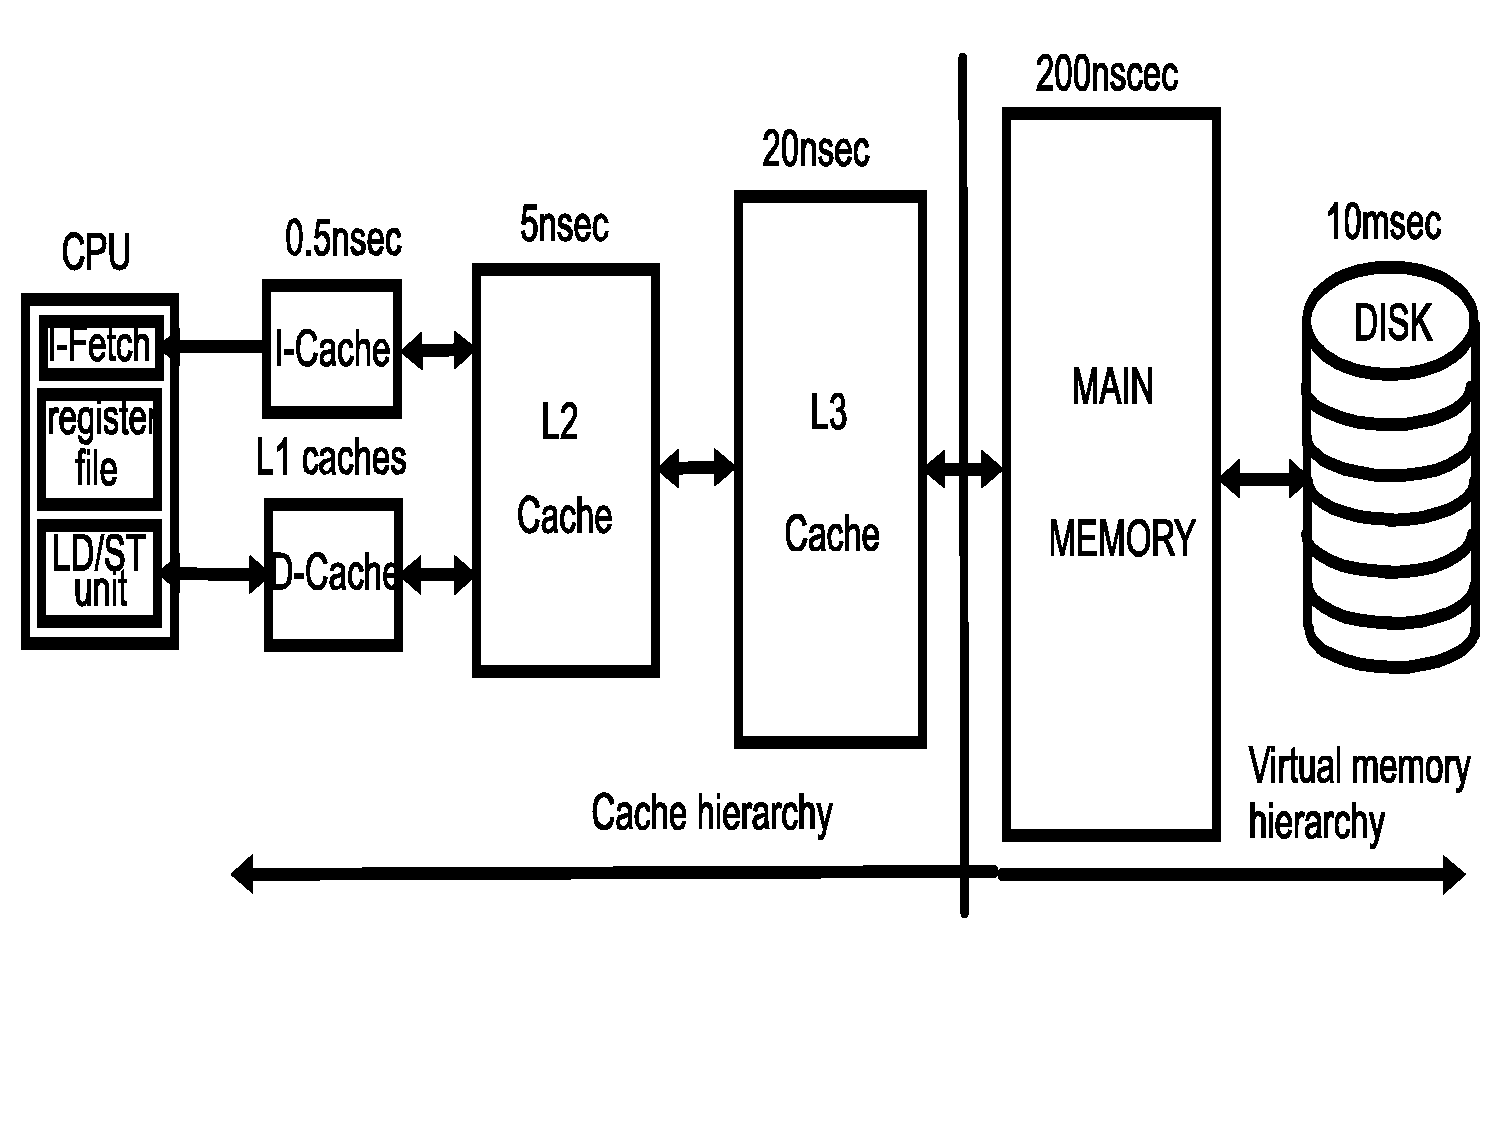
\includegraphics[width=44ex]{FigsMemH/MemHierarchy}
\column{0.30\textwidth}
\emph{Memory goes at electronic speed}, \emp{Disk at mechanical speed.}
\end{columns}
\vspace{-5ex}

\pause
\emph{Locality Principle:}\pause
\begin{itemize}
    \begin{scriptsize}
    \item small set of addresses accessed at a time, 
            named \emph{working set}, $\Rightarrow$ low miss rate,
    \item when program transitions $\Rightarrow$ abrupt change of working sets 
            $\Rightarrow$ high miss rate,
    \item \emph{Temporal Locality:} a referenced item is likely to be accessed again soon,
    \item \emph{Spatial Locality:} items close-by a referenced item likely to be accessed soon,
    \item \emph{Spatial $\Rightarrow$ Temporal} at block/page level.
    \end{scriptsize} 
\end{itemize}
\end{frame}

\begin{frame}[fragile,t]
\frametitle{Typical Memory Hierarchy}

\begin{columns}
\column{0.6\textwidth}
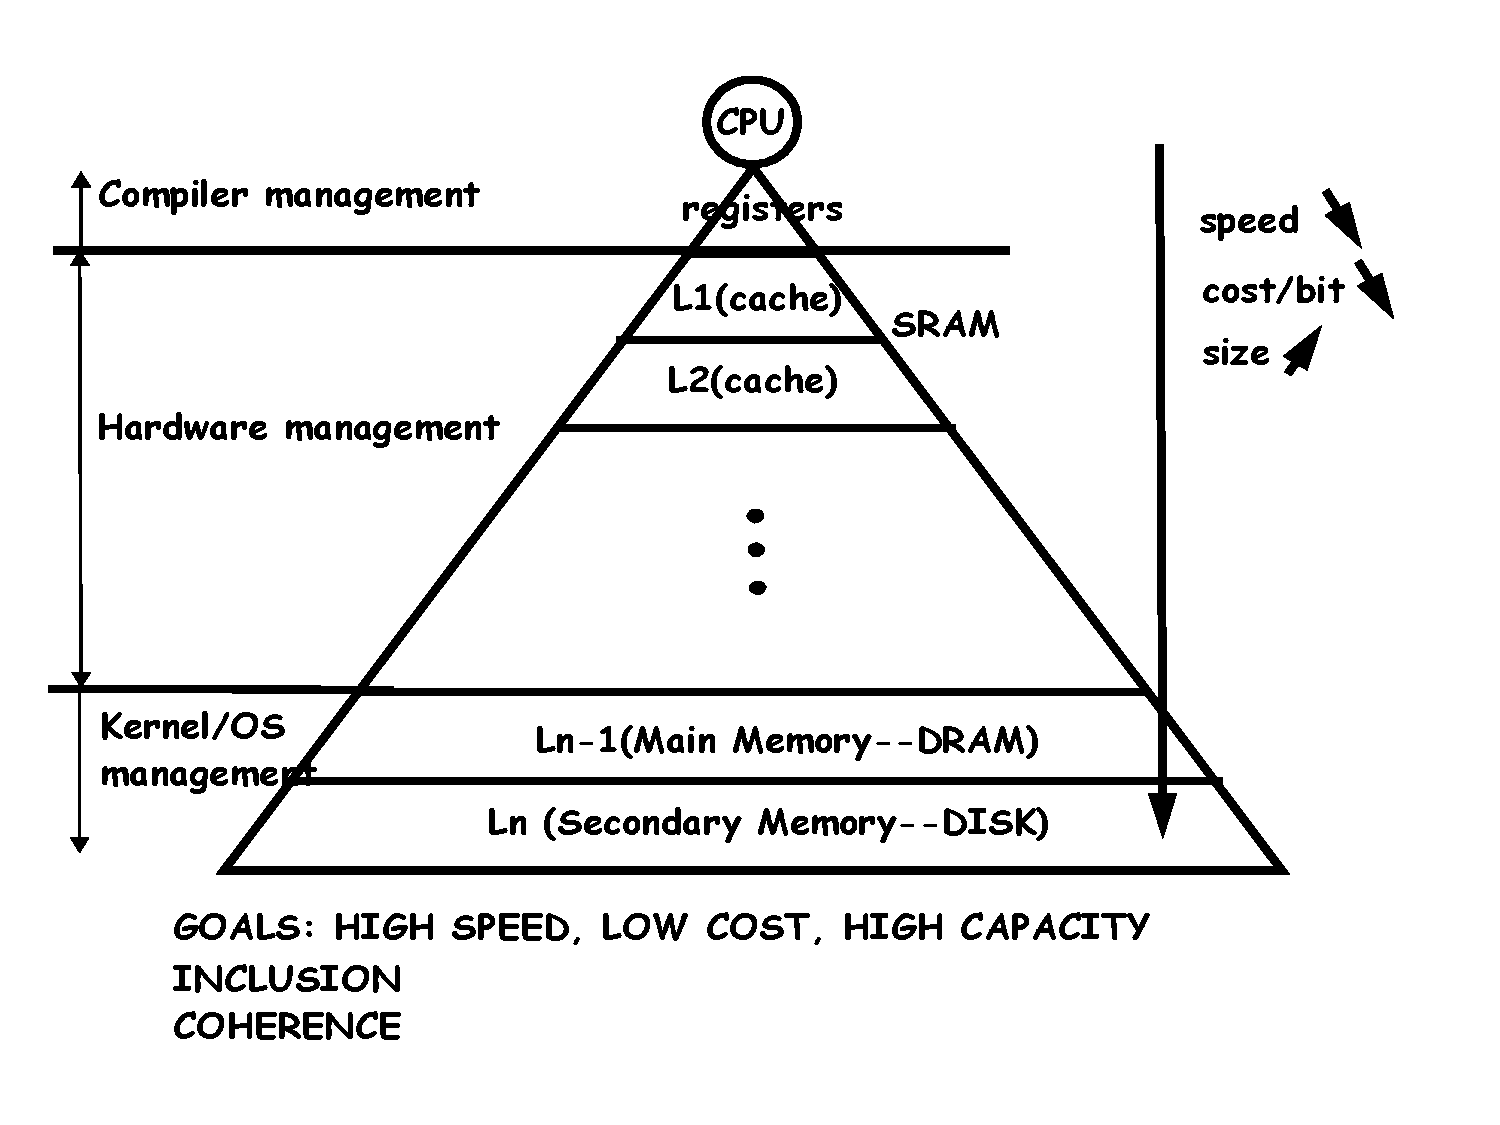
\includegraphics[width=44ex]{FigsMemH/Pyramid}
\column{0.37\textwidth}
\pause
\begin{scriptsize}
\begin{itemize}
\item \emph{Illusion of a monolithic memory of lowest cost, largest capacity \&
            fastest average access time.}\\
\smallskip
\item \emp{Larger caches are slower} because speed dominated by wire delays
    (do not scale with technology).
\end{itemize}
\end  {scriptsize}
\end{columns}

\begin{itemize}
\begin{scriptsize}
    \item \emp{Inclusion:} {\tt j > i} $\Rightarrow$ locations at level {\tt i} are also cached \& has same or more restrictive rights than level {\tt j}. Level-{\tt i} cache needs not be looked up if block not present at level {\tt j}.
    \item \emp{Coherence} for single cores: instrs executed out of order \& speculatively, but
            the result is as if instrs executed one at a time in program order \& monolithic memory.     
\end{scriptsize}
\end{itemize}
\end{frame}

%%%%%%%%%%%%%%%%%%%%%%%%%%%%%%%%%%%%%%%%%%%%%%%%%%%
%%%%%%%%%%%%%%%%%%%%%%%%%%%%%%%%%%%%%%%%%%%%%%%%%%%
%%%%%%%%%%%%%%%%%%%%%%%%%%%%%%%%%%%%%%%%%%%%%%%%%%%
\section{Cache (Hierarchy) Design}

\subsection{Performance Measures}
\begin{frame}[fragile,t]
\frametitle{Cache Performance}

\begin{itemize}
\begin{scriptsize}
\item \emp{Average Memory Access Time} ({\tt AMAT}):\\
        {\tt AMAT $=$ hit time + miss rate $\times$ miss penalty}\bigskip

\item \emp{Miss Rate $\equiv$ 1.0 - Hit Rate} $\equiv$ \% of accesses not satisfied at highest level:\\
        {\tt Miss Rate $\equiv$ (\# misses in L1) / (\# processor references)}  \bigskip

\item Misses Per Instruction ({\tt MPI}):\\
        {\tt MPI $=$ (\# misses in L1) / (\# instructions)}\\
        \emph{Easier to use than Miss Rate:} {\tt CPI $=$ CPI$_0$ + MPI$\times$MissPenalty}\\\bigskip

\item \emp{Miss Penalty}: average delay per miss caused in the processor:\\
        If processor blocks on misses $\Rightarrow$ miss latency (time to bring a block from mem)\\
        In an OoO processor cannot be measured directly $\neq$ miss latency\\\bigskip
\item \emp{Miss Rate and Penalty} can be defined at every cache level. Normalized to:\\
            \# of processor references or\\
            \# of accesses from the lower level.
\end  {scriptsize}
\end{itemize}

\end{frame}

\subsection{Cache Mappings}

\begin{frame}[fragile,t]
\frametitle{Cache Mapping}
 
\begin{itemize}
    \item Cache behavior mostly dictated by: cache size and
    \item {\bf The mapping} of \emp{memory blocks} to \emph{cache lines}.\\
            (Each cache line hosts multiple mem blocks at different times.)
    \item {\em direct or set-associative or fully-associative mapping}.\smallskip
\end{itemize}
\begin{columns}
\column{0.45\textwidth}
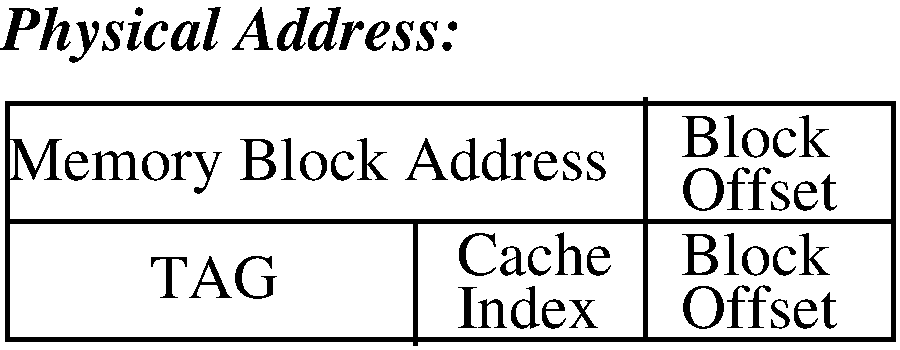
\includegraphics[width=25ex]{FigsMemH/CacheMapping}
\column{0.50\textwidth}
\begin{scriptsize}
Cache Acess Has Two Phases:
\begin{itemize}
    \item[cache index] use index bits to fetch {\tt tags} and data from the set,
    \item[tag check] check {\tt tag} to detect hit/miss (and status bits).
\end{itemize} 
\end  {scriptsize}
\end{columns}

\bigskip
Cache:
\begin{itemize}
    \item \emph{Data Memory}, i.e., the cached copy of the memory block + 
    \item \emp{Directory Memory}, one entry per cache line containing\\ 
            {\tt TAG} ({\tt ID}) \& status bits: valid, dirty, reference, cache coherence.\\\smallskip
\end  {itemize}

\end{frame}

\begin{frame}[fragile,t]
\frametitle{Direct-Mapped Cache}
 
{\em Cache Slicing:} a memory block mapped always in (the same) cache line, of index:
{\tt (Block Address) mod (\# of cache lines)}.\bigskip
\vspace{-3ex}
\begin{columns}
\column{0.65\textwidth}
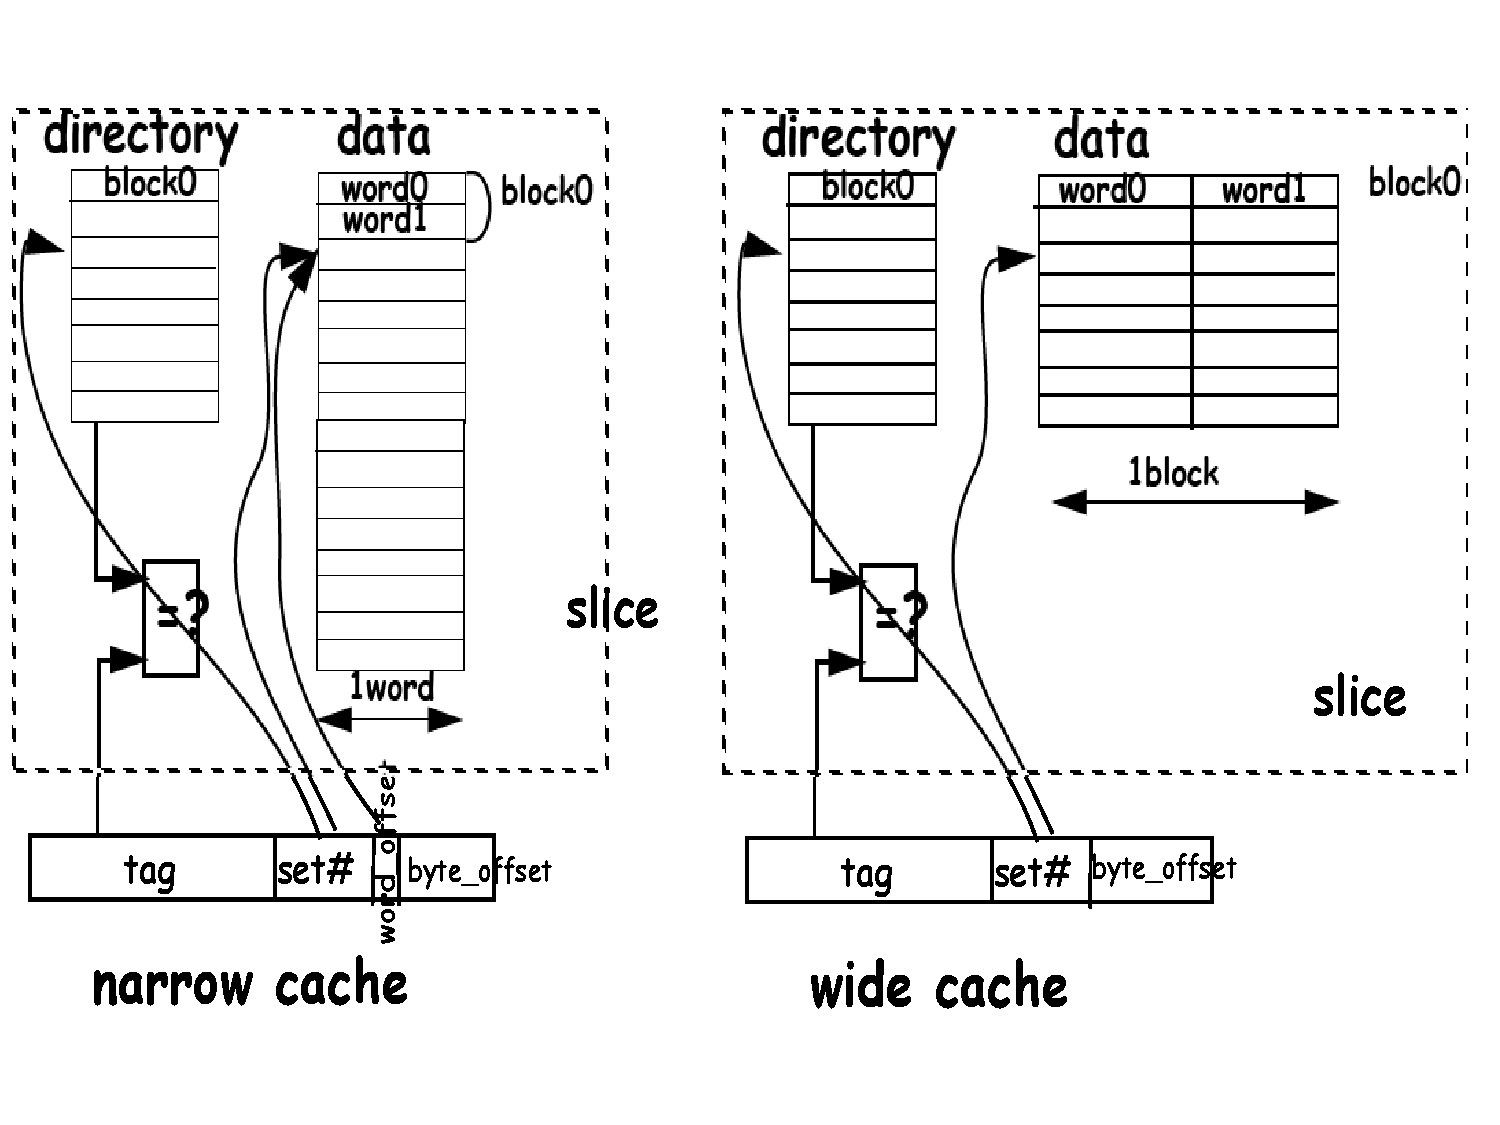
\includegraphics[width=44ex]{FigsMemH/CacheWide}
\column{0.32\textwidth}
\begin{scriptsize}
{\bf Two Phases:}\\
\emp{Index} + \emph{Tag Check}
\bigskip

\emp{Data-Entry Size:}\\ 
\begin{itemize}
    \item narrow (1 word) $\rightarrow$\\wide (1 cache line)
    \item[wide:] on a miss, the data is reloaded in one cycle of data mem.
    \item[narrow:] less complexity.
\end{itemize} 
\end  {scriptsize}
\end{columns}

\begin{itemize}
    \item[\emph{+}]  fast access time on a hit
    \item[\alert{-}] several blocks competing on the same line $\Rightarrow$ high miss rate 
\end  {itemize}

\end{frame}


\begin{frame}[fragile,t]
\frametitle{Set-Associative Cache}
 
Cache is partitioned into a set of lines:
\begin{itemize}
    \item \emp{access to each set is directly mapped}, but
    \item \emph{a block mapped to a set can reside anywhere in the set}!
\end  {itemize} 

\begin{itemize}
    \item[read] requires one cycle: all 3 directory and data entries fetched in {\tt ||},\\
                then the tag is compared in {\tt ||} with the tag bits of each slice\\
                a hit selects the corresponding word, all misses $\Rightarrow$ cache miss! 
    \item[write] requires at least two mem cycles (can be pipelined): one to check the hit or miss, 
                and then one to write into data memory. 
                 
\end  {itemize}


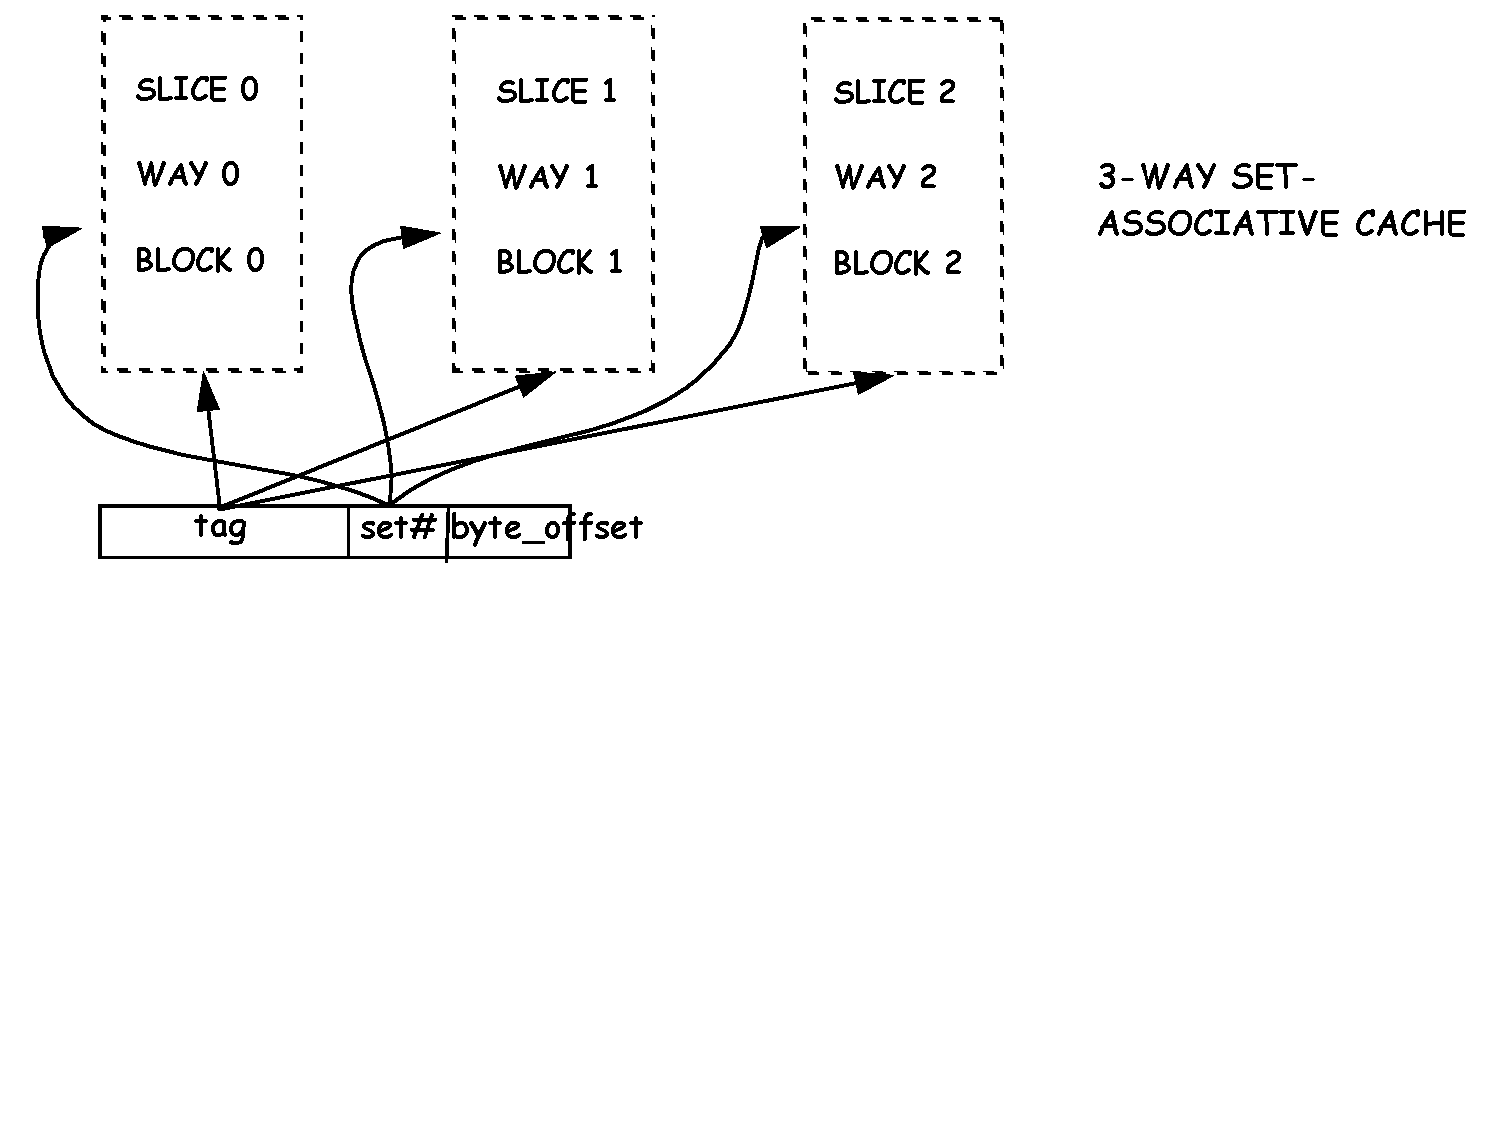
\includegraphics[width=55ex]{FigsMemH/SetAssoc}

\end{frame}


\begin{frame}[fragile,t]
\frametitle{Full-Associative Cache}
 
Very different structure than an all-way set-associative cache:\\
to find the block all directories must be checked in {\tt ||}!

\begin{columns}
\column{0.4\textwidth}
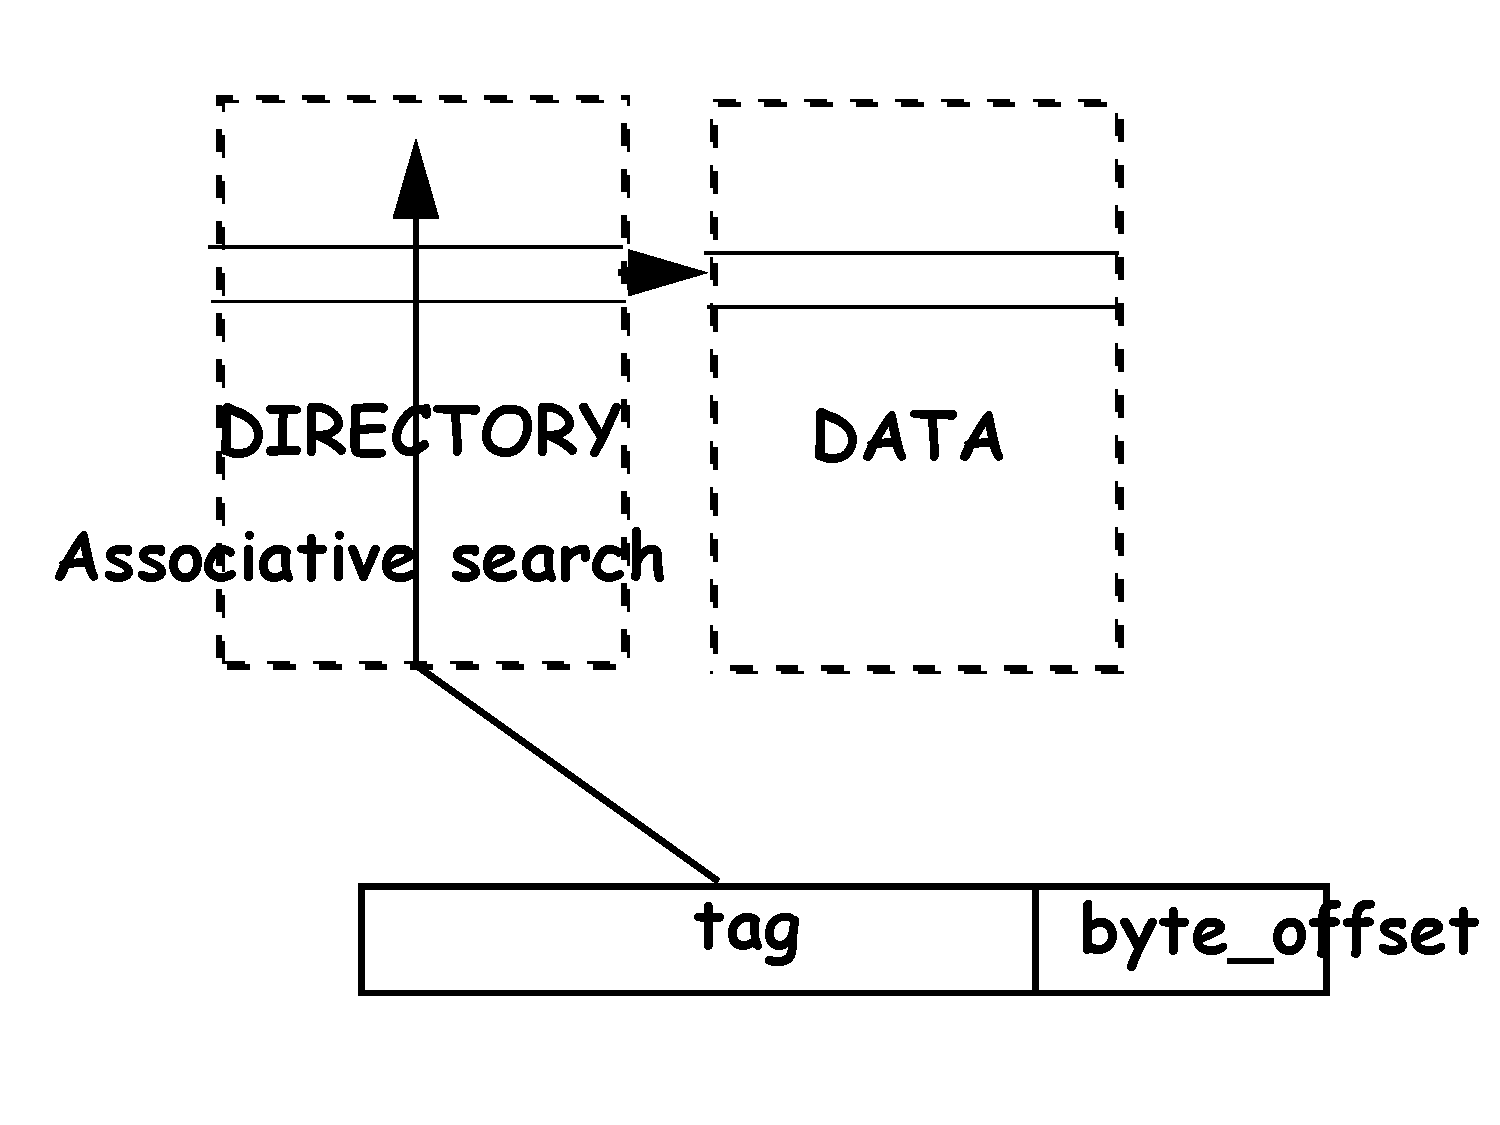
\includegraphics[width=33ex]{FigsMemH/FullAssoc}\pause
\column{0.55\textwidth}
%\begin{scriptsize}
Two Steps:
\begin{itemize}
    \item \emp{{\tt||} tag check} $\Rightarrow$ tag bus lines throughout the directory; 
            comparator associated with each dir entry, then
    \item  \emph{on match} the row line is activated and data returned.
\end  {itemize} 
%\end{scriptsize}
\end{columns}

Content-Addressable Memory (CAM) \emp{slower \& less dense} than RAM.\\
(signal propag, comparison, etc.)\bigskip

Small Caches: fully associative because potential for conflict in hot sets
    is damaging to performance. 

\end{frame}

\subsection{Replacement Policies}
\begin{frame}[fragile,t]
\frametitle{Replacement Policies (Selects a Victim Block)}

Random, Least Recently Used (LRU), FIFO, Pseudo-LRU:\\
    {\tt~~~~}maintain replacement bits.

\vspace{-2ex}
\begin{columns}
\column{0.7\textwidth}
\hspace{-5ex}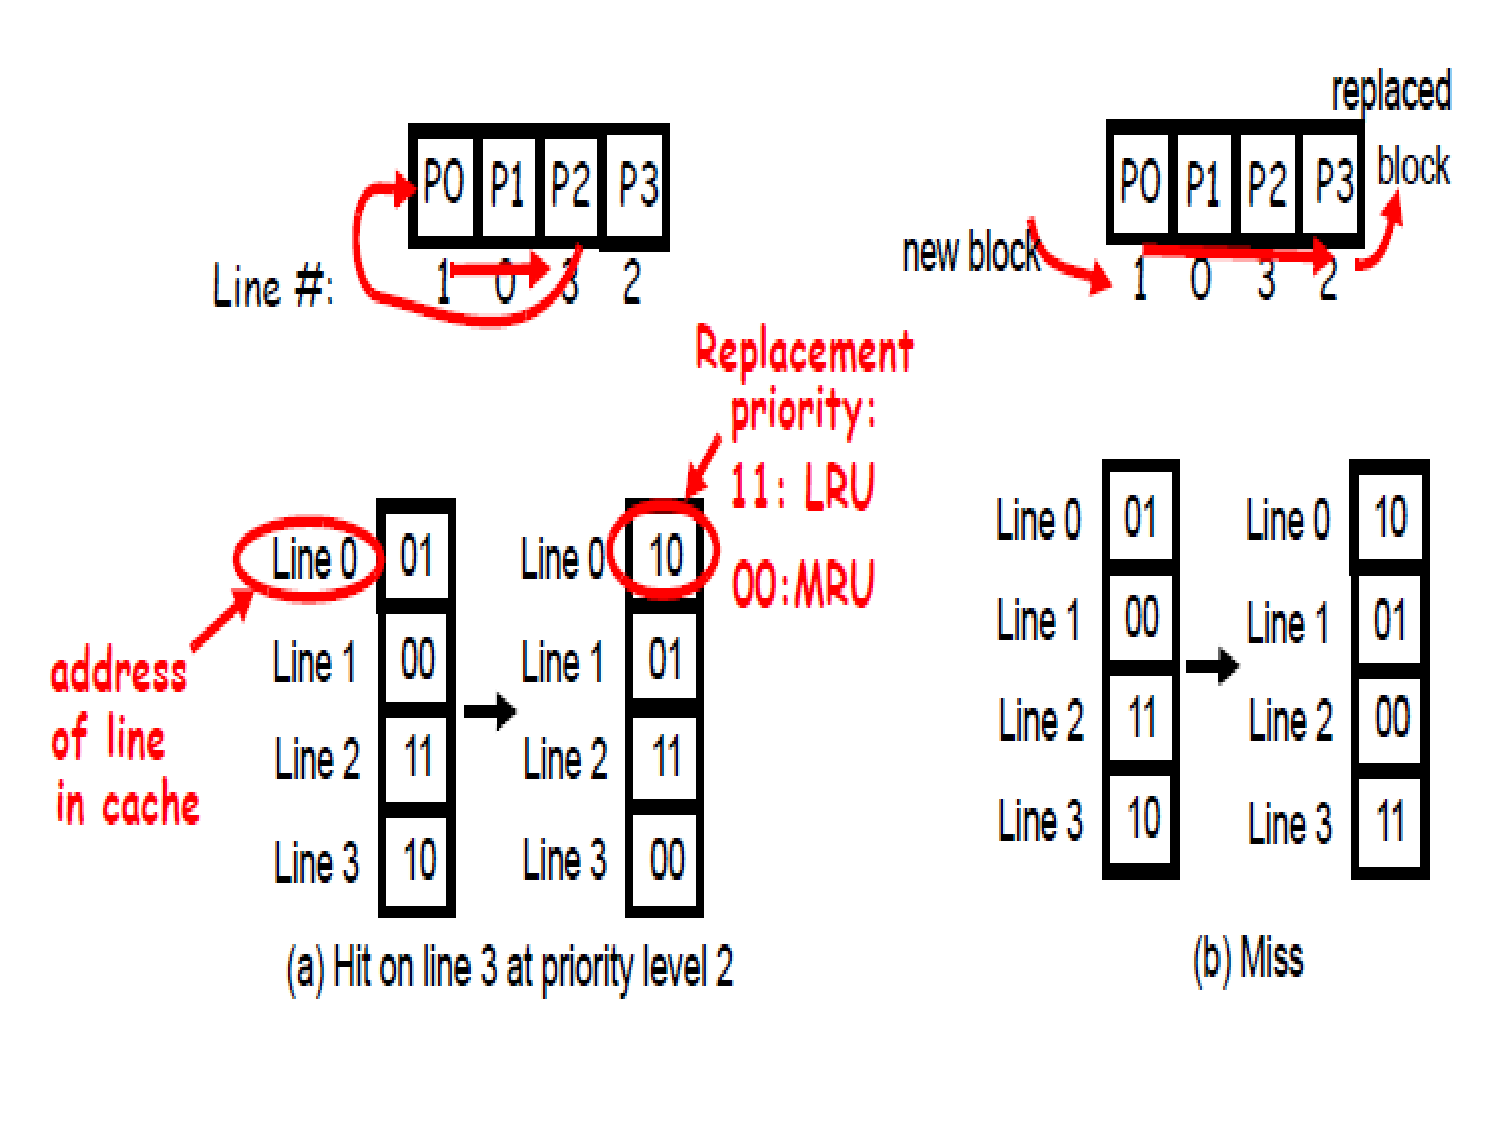
\includegraphics[width=50ex]{FigsMemH/LRU}\pause
\column{0.2\textwidth}
$\Leftarrow$ LRU Example:
\end{columns}
\vspace{-2ex}
\emp{Direct Mapper $\Rightarrow$ No Need.}\\
\emp{Set/Fully Associative $\Rightarrow$ Per-Set/Cache Replacement.}

\end{frame}


\subsection{Write (Through/Back) Policies}
\begin{frame}[fragile,t]
\frametitle{Write Policies}

%\emp{Write Through} to next level on all writes
\begin{columns}
\column{0.51\textwidth}
\hspace{-4ex}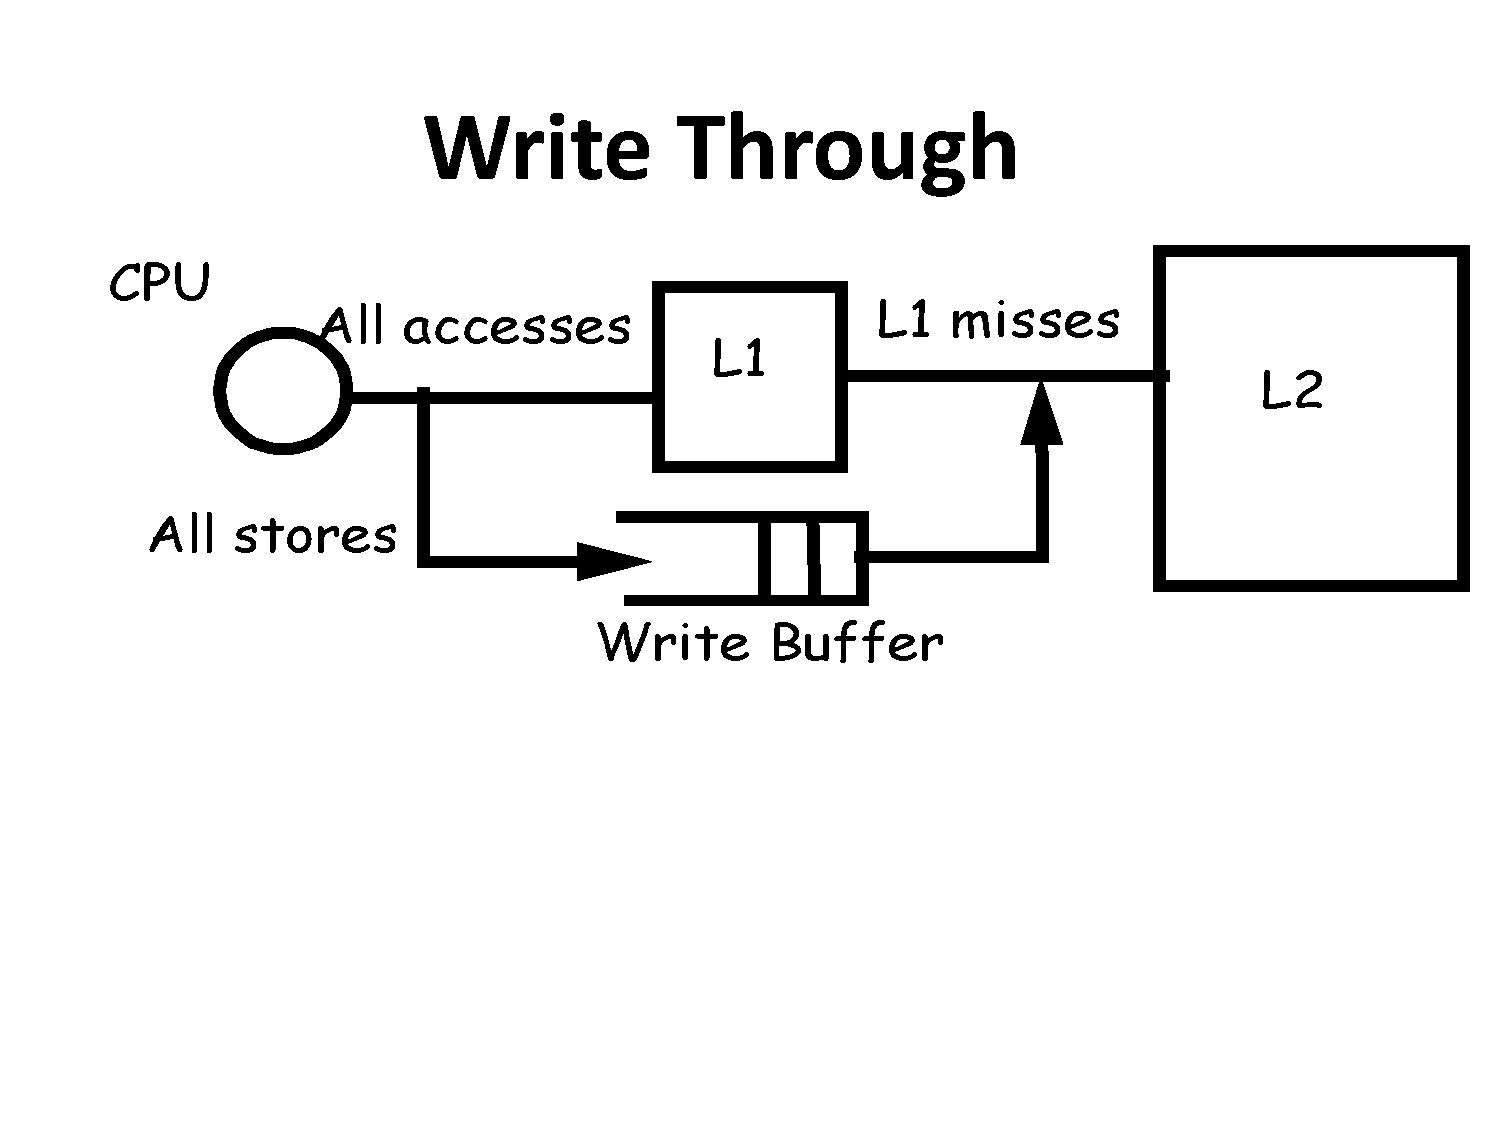
\includegraphics[width=40ex]{FigsMemH/WriteThrough}
\column{0.46\textwidth}
\vspace{-8ex}
\begin{itemize}
\begin{scriptsize}
    \item {\bf write to next level on all writes}
    \item use a write buffer to avoid stalls;\\
            loads must check the buffer first!
    \item Used for small 1st-level caches: 
    \item \emph{simple, no inconsistency on levels}
    \item but \emp{large store traffic}
\end  {scriptsize}
\end  {itemize}
\end{columns}

\vspace{-8ex}
\begin{columns}
\column{0.44\textwidth}
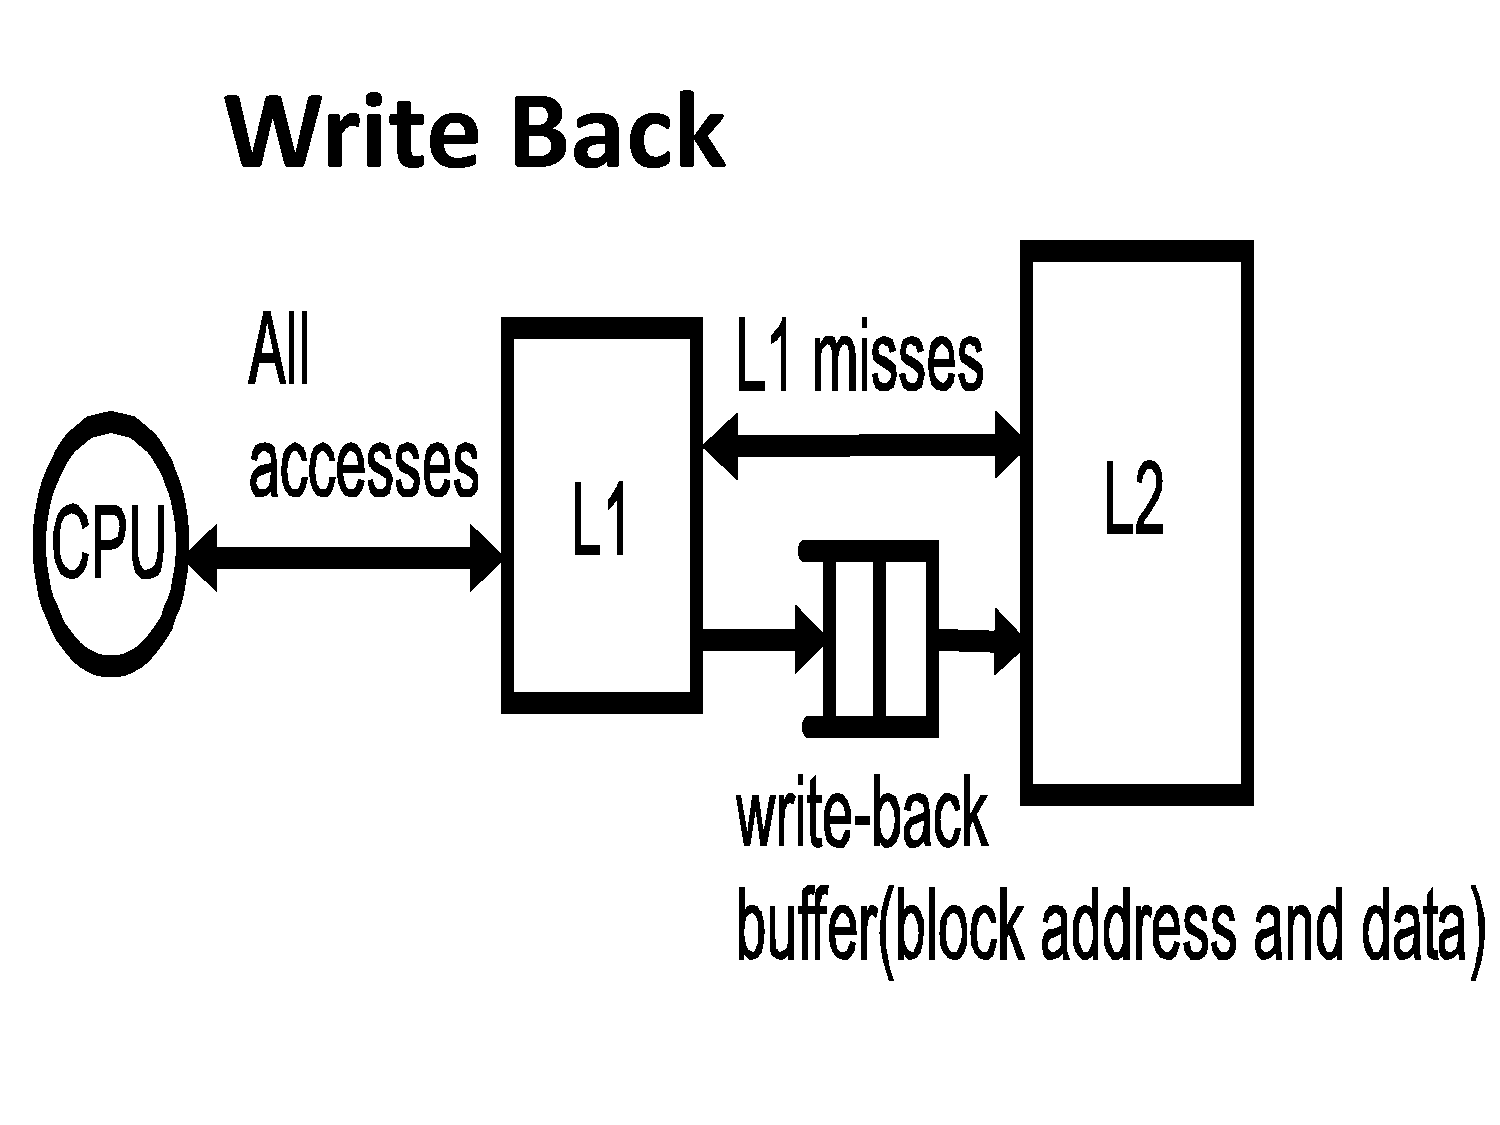
\includegraphics[width=35ex]{FigsMemH/WriteBack}
\column{0.53\textwidth}
\vspace{-3ex}
\begin{itemize}
\begin{scriptsize}
    \item {\bf write to next level on replacement}
    \item uses a dirty bit ({\tt db}) \& write-back buffer\\
            block is loaded/modified $\Rightarrow$ {\tt db} reset/set\\
            block is evicted $\Rightarrow$ if {\tt db} set then written.
    \item \emph{write happens only on a miss}\smallskip

    \item IN BOTH CASES: a load checks the buffer first (consistency)!
    \item Write Miss: always allocate on write back; design choice in write through!
%    \item On a write miss: (i) Write-Back always allocates; (ii) design choice in write through. 
\end  {scriptsize}
\end  {itemize}\bigskip
\end{columns}
\end{frame}


\subsection{The Four Types of Cache Misses}
\begin{frame}[fragile,t]
\frametitle{Classification of Cache Misses}

The Four C's:
\begin{itemize}
\begin{scriptsize}
\item[Cold] (Compulsory) misses: first reference of a block,\smallskip

\item[Capacity] misses: insufficient space for data/code,\smallskip

\item[Conflict] misses: two memory blocks map to the same cache line,\smallskip

\item[Coherence] misses, e.g., another thread has modified the needed value.\bigskip
\end  {scriptsize}
\end{itemize}

How to measure them:
\begin{itemize}
\begin{scriptsize}
\item[Cold:] simulate infinite cache size,\smallskip

\item[Capacity:] simulate fully-assoc cache and subtract cold misses\smallskip

\item[Conflict:] simulate cache and subtract cold and capacity misses.\bigskip
\end  {scriptsize}
\end{itemize}

\end{frame}


\begin{frame}[fragile,t]
\frametitle{Multi-Level Cache Hierarchies}

\begin{columns}
\column{0.65\textwidth}
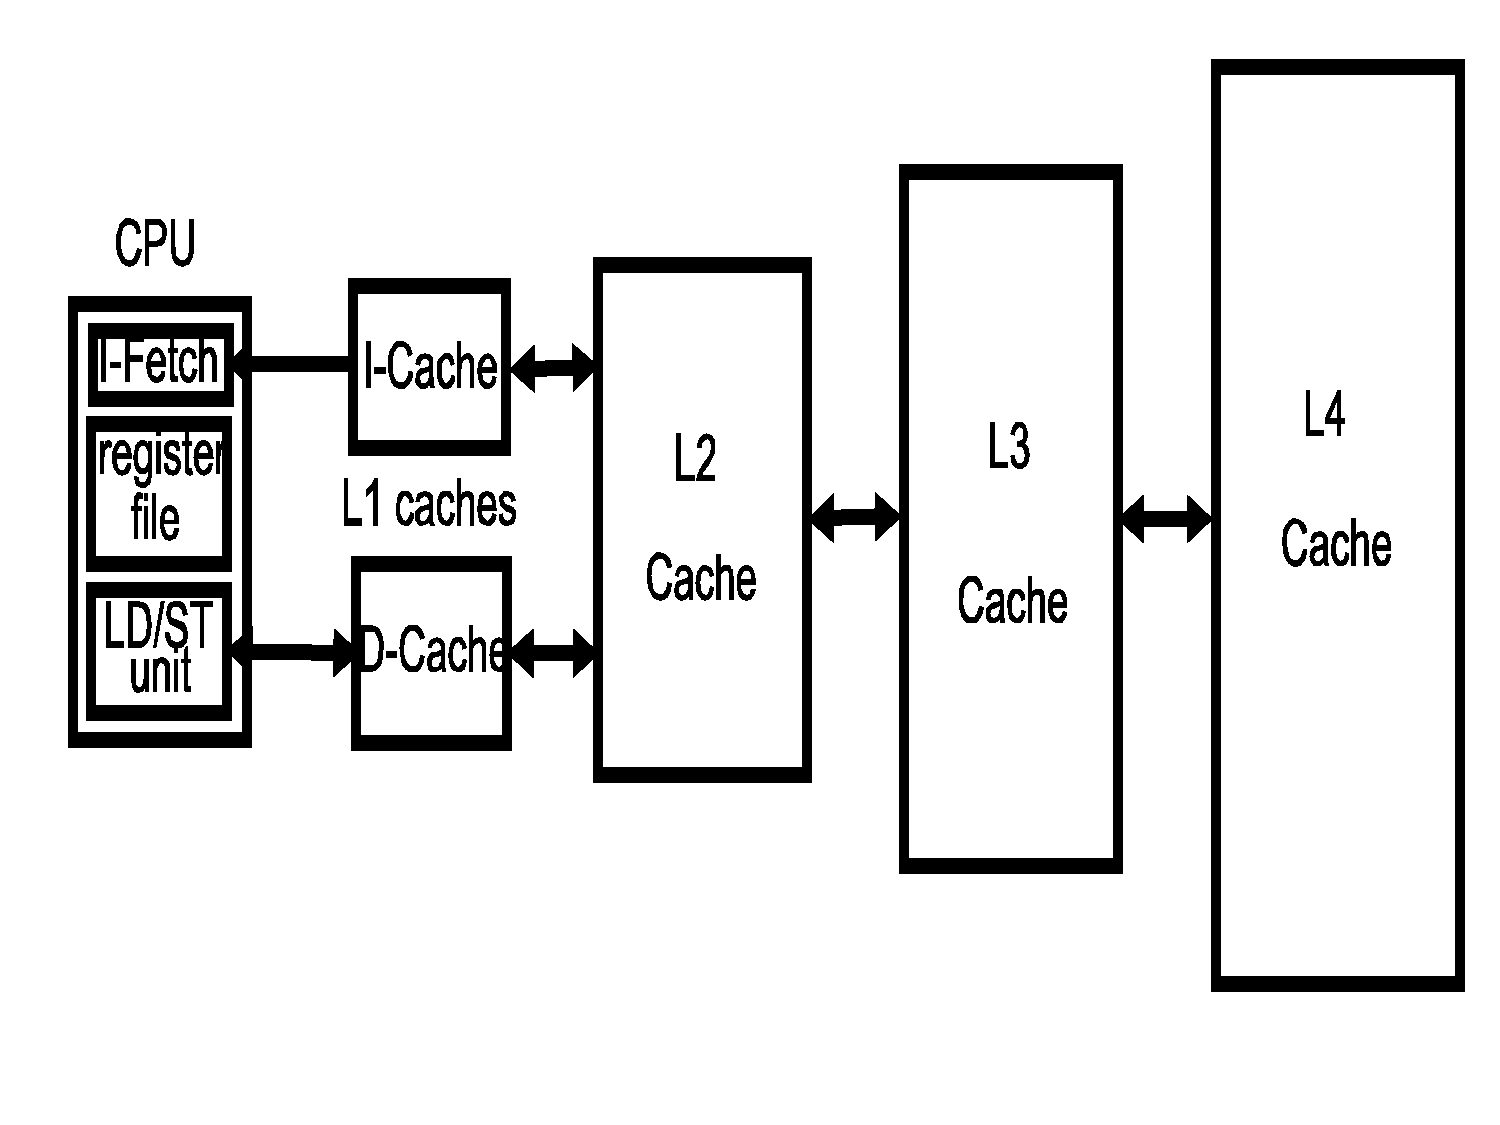
\includegraphics[width=35ex]{FigsMemH/MultiLevCache}
\column{0.3\textwidth}
1st and 2nd levels on chip; 3rd and 4th mostly off chip\smallskip
\end{columns}

We will assume \emph{Cache Inclusion}. A block
\begin{scriptsize}
\begin{itemize}
    \item misses in $L_i$ $\Rightarrow$ must be brought in all $L_j, j>i$.
    \item is replaced in $L_j$ $\Rightarrow$ must be removed in all $L_i, j>i$.
    \item \emp{replication} but \emph{good for coherence}.
\end  {itemize}
\end  {scriptsize}\bigskip

\emp{Cache Exclusion.} A block:
\begin{scriptsize}
\begin{itemize}
    \item is in $L_i$ $\Rightarrow$ then it is not in any other level.
    \item misses in $L_i$ $\Rightarrow$ all copies are removed from all levels $> i$.
    \item is replaced in $L_j$ $\Rightarrow$ allocated in $j+1$.
    \item \emph{size is the sum of all caches}, but \emp{horrible for coherence}.
\end  {itemize}
\end  {scriptsize}\bigskip

\end{frame}


\begin{frame}[fragile,t]
\frametitle{Cache Parameters}

Large Caches: slower (wire delays), more complex, less capacity misses.\bigskip

Larger Block Size: 
\begin{itemize}
    \item exploits spatial locality, but
    \item if too big $\Rightarrow$ capacity misses $\uparrow$
    \item big blocks increase miss penalty.\bigskip
\end  {itemize}

Higher Set Associativity (SA): 
\begin{itemize}
    \item addresses conflict misses
    \item 8-16 ways SA as good as fully associative
    \item A 2-way SA cache of size $N$ has similar 
            miss rate with a direct mapped of size $2\times N$.
    \item Higher hit time.
\end  {itemize}
\end{frame}

\section{Improving Cache Performance}

\subsection{Lockup-Free Caches}

\begin{frame}[fragile,t]
\frametitle{Lockup-Free Caches}

\begin{columns}
\column{0.5\textwidth}
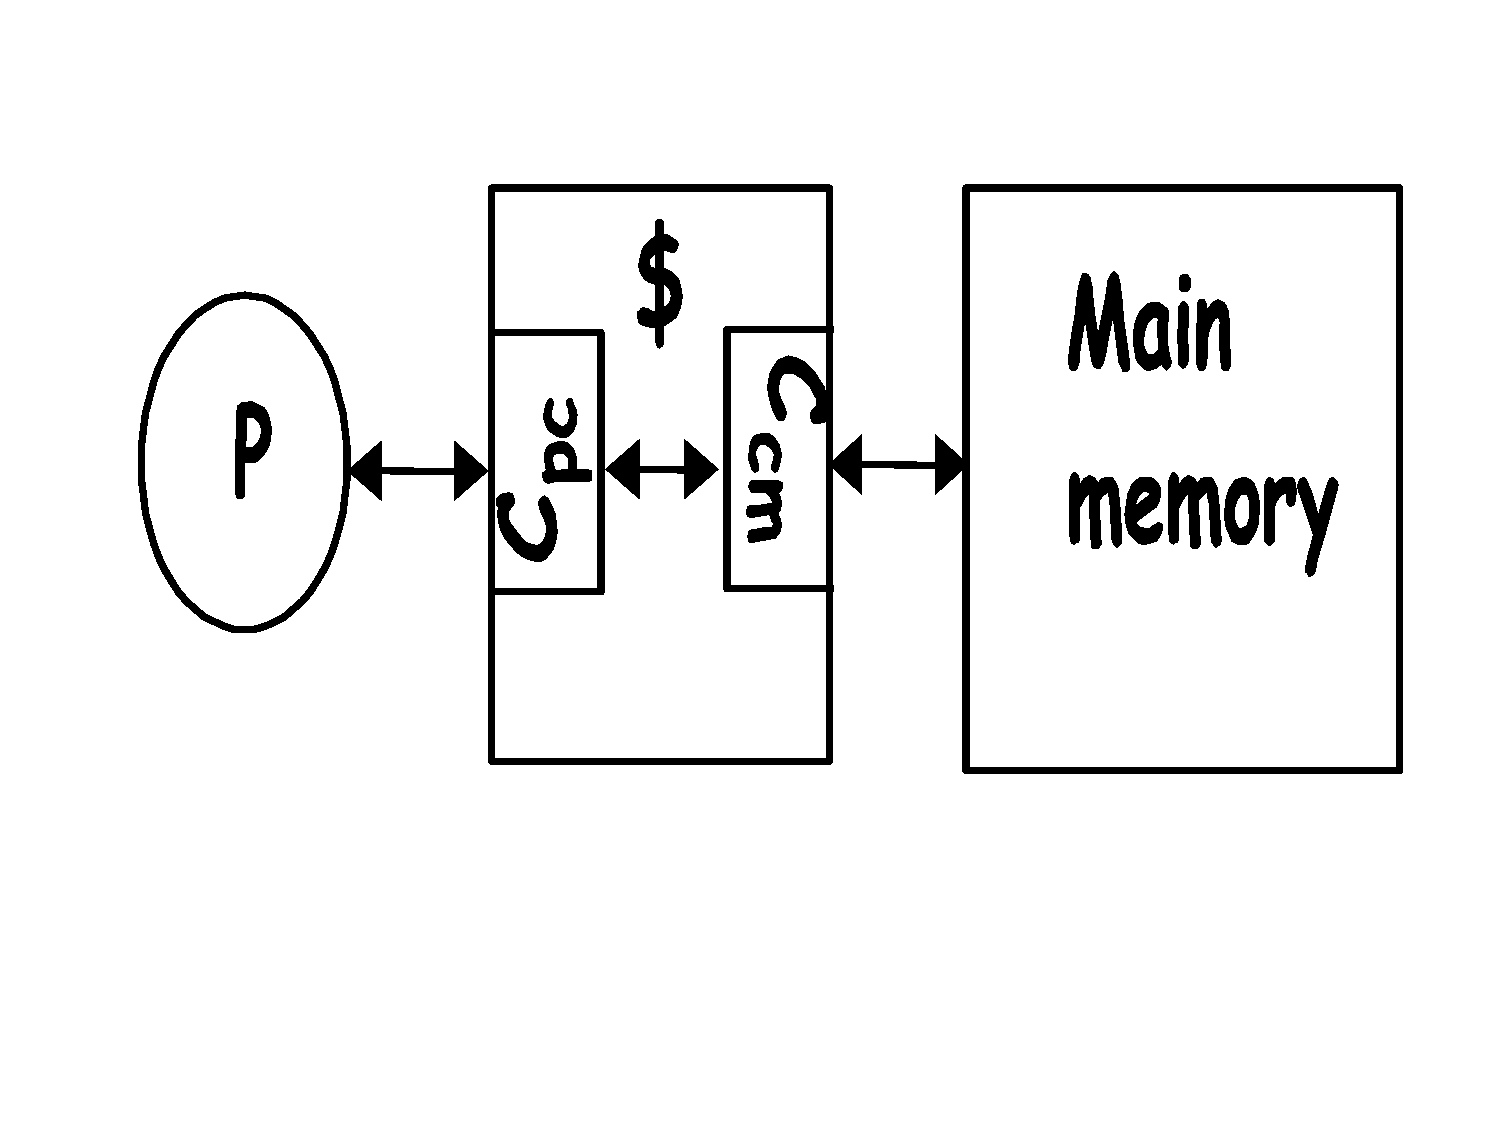
\includegraphics[width=35ex]{FigsMemH/CpcCcm}
\column{0.47\textwidth}
Cache is a Two-Ported Device:\\
Memory \& Processor.\smallskip

$C_{pc}:$ cache to processor interf\smallskip

$C_{cm}:$ cache to memory interface
\end{columns}
\vspace{-3ex}

\begin{itemize}
\begin{scriptsize}
    \item Needed to support Prefetching \& Dynamically-Scheduled OoO Single Proces 
            \& Core MultiThreading \& Multi Cores
    \item A Lockup-Free Cache does not block on a miss, but keeps accepting proc requests,
    \item hence, it allows concurrent processing of multiple hits/misses.
    \item Cache has to bookkeep all pending misses:
        \begin{itemize}
        \begin{scriptsize}
            \item Miss Status Handling Register ({\tt MSHR}) contains 
                    address of the pending miss $+$ destination block in cache $+$ 
                    destination register.
            \item {\tt MSHR} used to complete a miss and 
                    to avoid sending multiple miss requests per block.
                    \# of {\tt MSHR}s limits the \# of pending misses (at a time).
        \end{scriptsize} 
        \end  {itemize}
    \item Data dependencies eventually block the processor.
\end {scriptsize}
\end  {itemize}
\end{frame}

\begin{frame}[fragile,t]
\frametitle{Lockup-Free Caches (Continuation)}


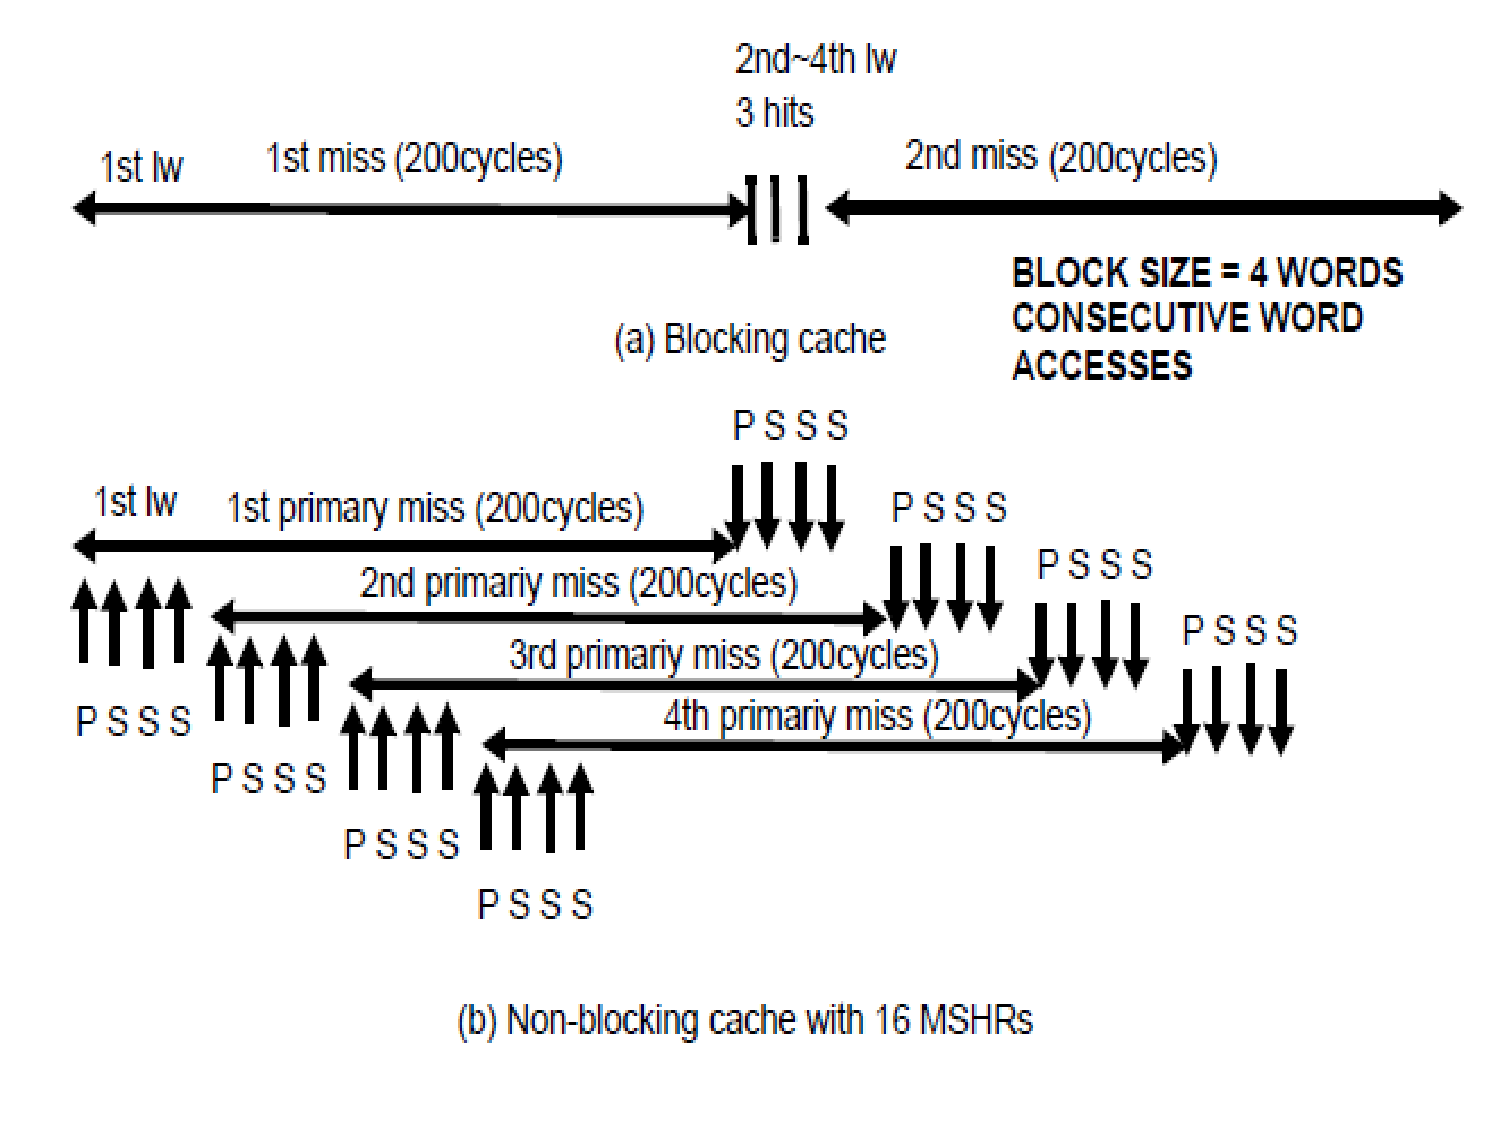
\includegraphics[width=44ex]{FigsMemH/PrimSecMiss}

\begin{itemize}
    \item Primary Miss (P) is the first miss to a block
    \item Secondary Miss (S) next accesses to same block {\scriptsize (due to pending P)} 
        \begin{itemize}
        \begin{scriptsize}
            \item Many more misses than Blocking Cache, which has only Ps.
            \item Needs {\tt MSHR}s for both P and S misses
            \item Misses are overlapped with computation and other misses.
        \end {scriptsize}
        \end  {itemize}
\end  {itemize}
\end{frame}

\subsection{Hardware/Software Prefetching}

\begin{frame}[fragile,t]
\frametitle{Hardware Prefetching}

\begin{columns}
\column{0.4\textwidth}
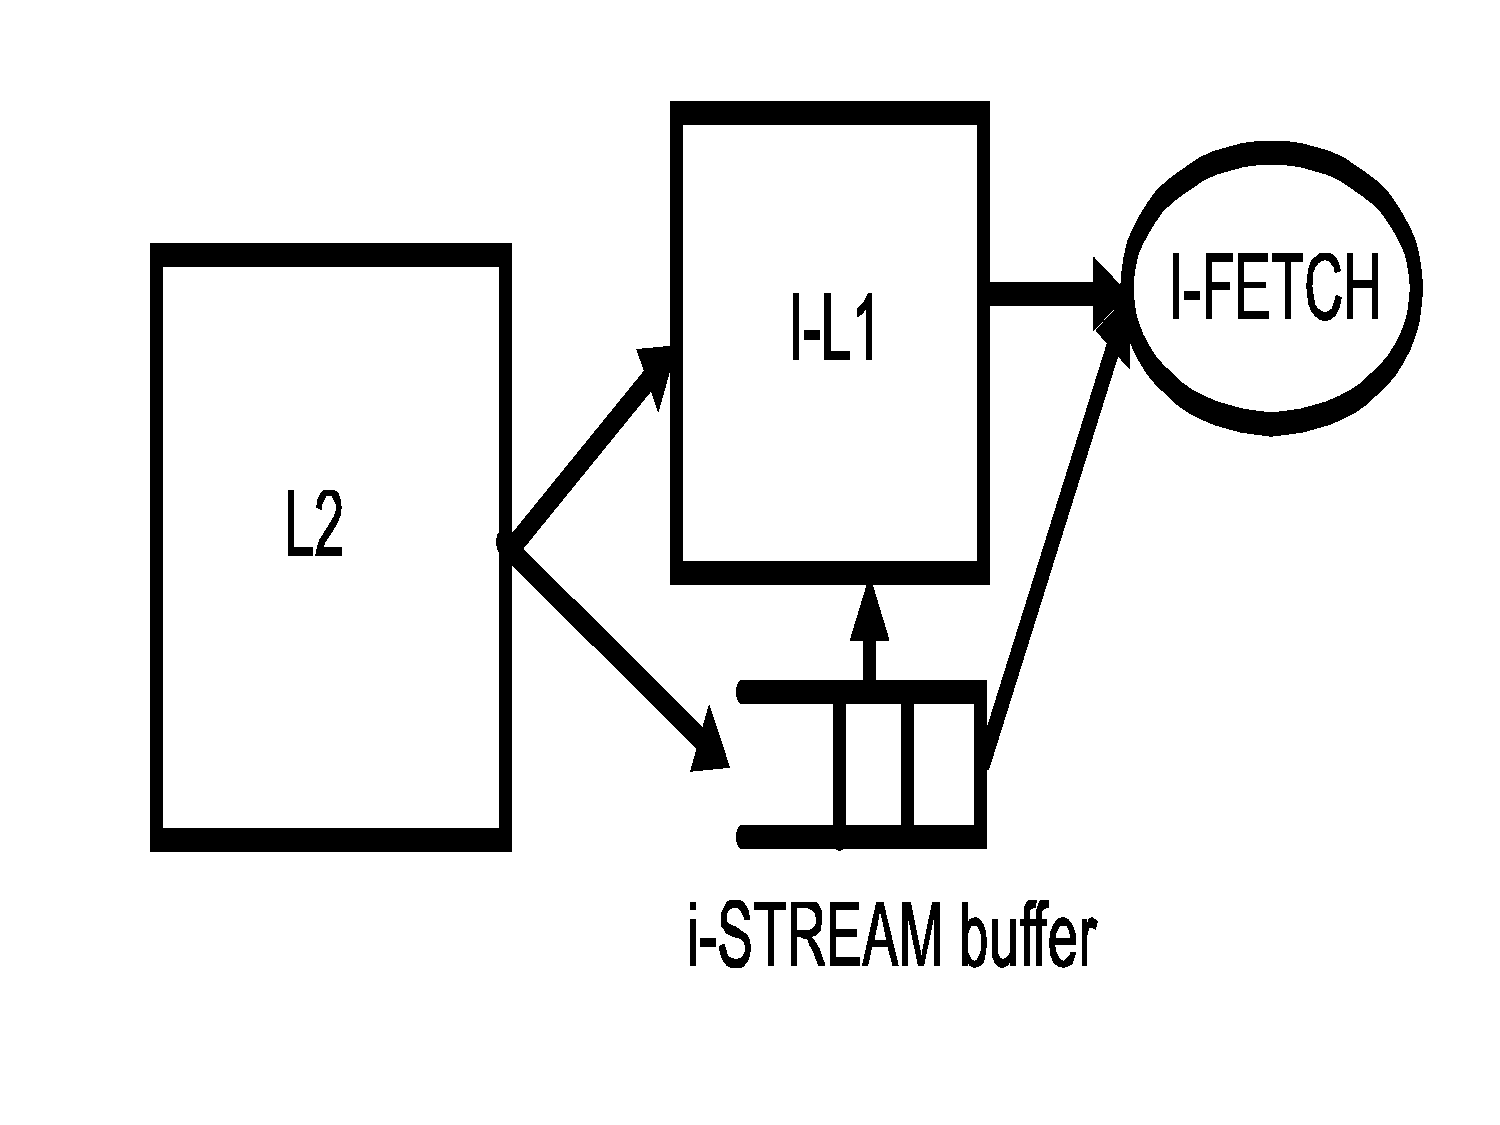
\includegraphics[width=27ex]{FigsMemH/SeqPrefetching}
\column{0.55\textwidth}
Sequential Prefetching Of Instrs:\smallskip
\begin{scriptsize}
I-Fetch Miss $\Rightarrow$ fetch 2 blocks instead of 1.\\\smallskip
2nd block stored in i-STREAM buffer:\\
(1) If I-STREAM hits $\Rightarrow$ block moved to L1\\
(2) Not accessed $\Rightarrow$ I-STREAM blocks overlaid.\\
(3) Prefetch Buffer avoids cache pollution.\\
(4) Applicable to data but less effective.
\end  {scriptsize}
\end{columns}

\begin{columns}
\column{0.45\textwidth}
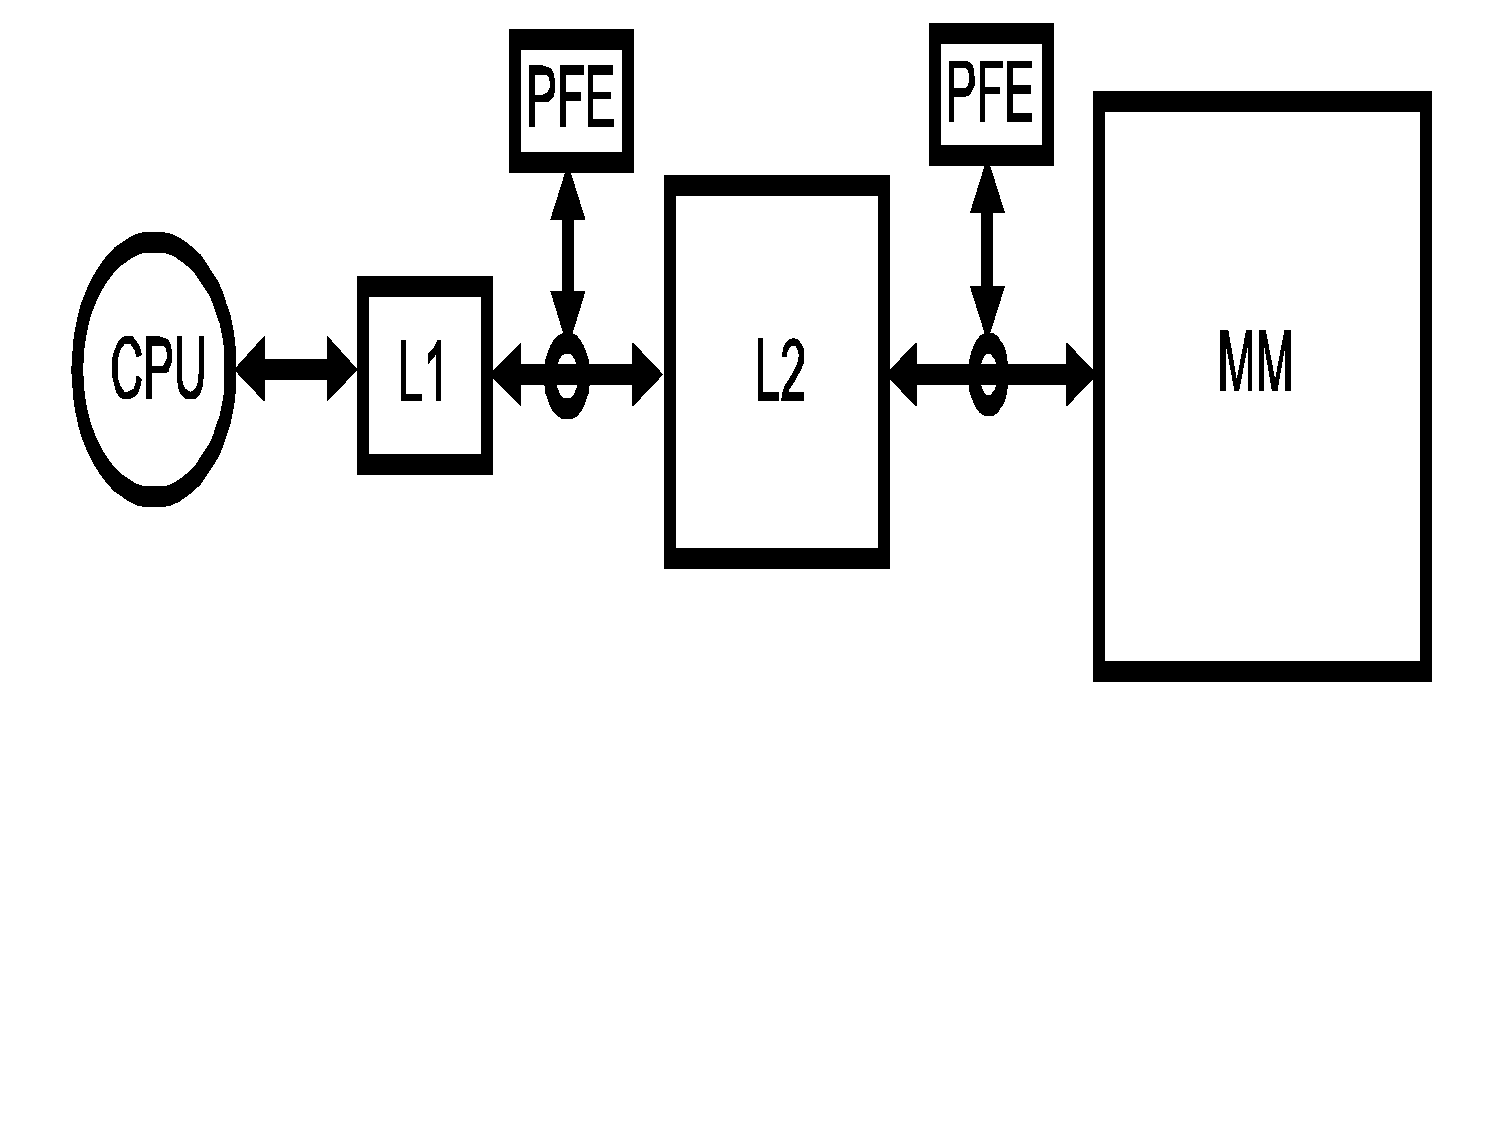
\includegraphics[width=33ex]{FigsMemH/HwdPrefetching}
\column{0.5\textwidth}
Hardware Prefetch Engines (PFE):\\\smallskip
\begin{scriptsize}
(1) detect strides in stream of missing\\ 
{\tt~~~}addresses by observing the bus then\\
{\tt~~~}start fetching ahead.\\
(2) naturally triggered by speculative exec:\\ 
(3) prefetch is harmless, i.e.,\\
{\tt~~~}exception $\Rightarrow$ prefetch dropped.\\
(4) but might polute caches.
\end  {scriptsize}
\end{columns}

\end{frame}


\begin{frame}[fragile,t]
\frametitle{Software Prefetching}

\begin{itemize}
    \item Prefetch instrs: non-blocking \& non-binding (load in-cache only)
    \item E.g., prefetch instructions may be inserted in the loop's body 
            to prefetch data needed by future iterations:
\end  {itemize}

\begin{block}{HL Code{\tt~~~~~~~~~~~}MIPS Code}\vspace{-2ex}
\begin{columns}
\column{0.18\textwidth}
\begin{colorcode}[fontsize=\scriptsize]
for(i=1000;i>0;i--)
  A[i]=A[i]+s
\end{colorcode} 
\column{0.40\textwidth}
\begin{colorcode}[fontsize=\scriptsize]
Loop: L.D   F2, 0(R1)
      PREF    -24(R1)
      ADD.D F4, F2, F0
      S.D   F4, 0(R1)
      SUBI  R1, R1, #8
      SUBI  R2, R2, #1
      BNEZ  R2, Loop
\end{colorcode} 
\column{0.35\textwidth}
{\tt PREF    -24(R1)}\\
prefetches the elements of {\tt A} 3 iterations ahead.
\end{columns}
\end{block}

\begin{itemize}
    \item Works for both load and stores, but
    \item data must be prefetched at perfect time:\\
            not too early (cache polution), not too late (not in cache),
    \item Instructional overhead \& requires non-blocking cache,
    \item Done for arrays, but also for pointer accesses.
\end  {itemize}
\end{frame}

\begin{frame}[fragile,t]
\frametitle{Faster Hit Times}

Princeton vs Harvard Cache:
\begin{itemize}
    \item Princeton: unified instr/data cache $\Rightarrow$ can use whole cache 
    \item Harvard: split instr/data cache $\Rightarrow$ optimized for access type.
    \item Pipelined Machine: FstLC Harvard \& SndLC Princeton.\bigskip
\end  {itemize}

Pipeline Cache Accesses:
\begin{itemize}
    \item Especially useful for stores:
    \item Pipeline Tag Check and Data Store (2 mem cycles)
    \item Separate Read/Write Ports to cache, optimized for each
    \item Also useful for I-Caches and Load in D-Caches
    \item $\uparrow$ pipeline length, but must split cache accesses into stages!
\end  {itemize}
\end{frame}


\begin{frame}[fragile,t]
\frametitle{Faster Hit Times (Continuation)}

Keep the cache simple and fast:\smallskip
\begin{itemize}
    \item Favors direct-mapped cache:
        \begin{itemize}
            \item less multiplexing
            \item overlap of tag and use of data.
        \end{itemize}\smallskip
    \item Interestingly, the size of FLC tends to decrease and
            associativity goes up as FLCs try to keep up with CPU.
\end  {itemize}

\begin{scriptsize}
\begin{tabular}{ll}
\hline
Processor    &  L1 Data Cache\\\hline
Alpha 21164  &  8KB, direct mapped\\\hline
Alpha 21364  &  64KB, 2-way\\\hline
MPC 750  &  32KB, 8-way, PLRU\\\hline
PA 8500  &  1MB, 4-way, PLRU\\\hline
Classic Pentium  &  16KB, 4-way, LRU\\\hline
Pentium-II  &  16KB, 4-way, PLRU\\\hline
Pentium-III  &  16KB, 4-way, PLRU\\\hline
Pentium-IV  &  8KB, 4-way, PLRU\\\hline
MIPS R10K/12K  &  32KB, 2-way, LRU\\\hline
UltraSparc-IIi  &  16KB, direct mapped\\\hline
UltraSparc-III  &  64KB, 4-way, random\\\hline
\end{tabular}
\end{scriptsize}
\end{frame}

\section{Virtual Memory}

\begin{frame}[fragile,t]
\frametitle{Why Virtual Memory?}

Allows applications to be bigger than Main Memory.\smallskip

Multiple Process Management:\smallskip
\begin{itemize}
    \item Each processor gets its own chunk of memory:
    \item Protection against each other,
    \item Protection against themselves,
    \item Application and CPU run in virtual space,
    \item Virtual-to-Physical Space Mapping invisible to application,
\end  {itemize}

%\bigskip
%Management between Main Memory (MM) and Disk:\\
%Miss in MM $\Rightarrow$ Page Fault
\end{frame}

\begin{frame}[fragile,t]
\frametitle{Virtual Address Mapping}
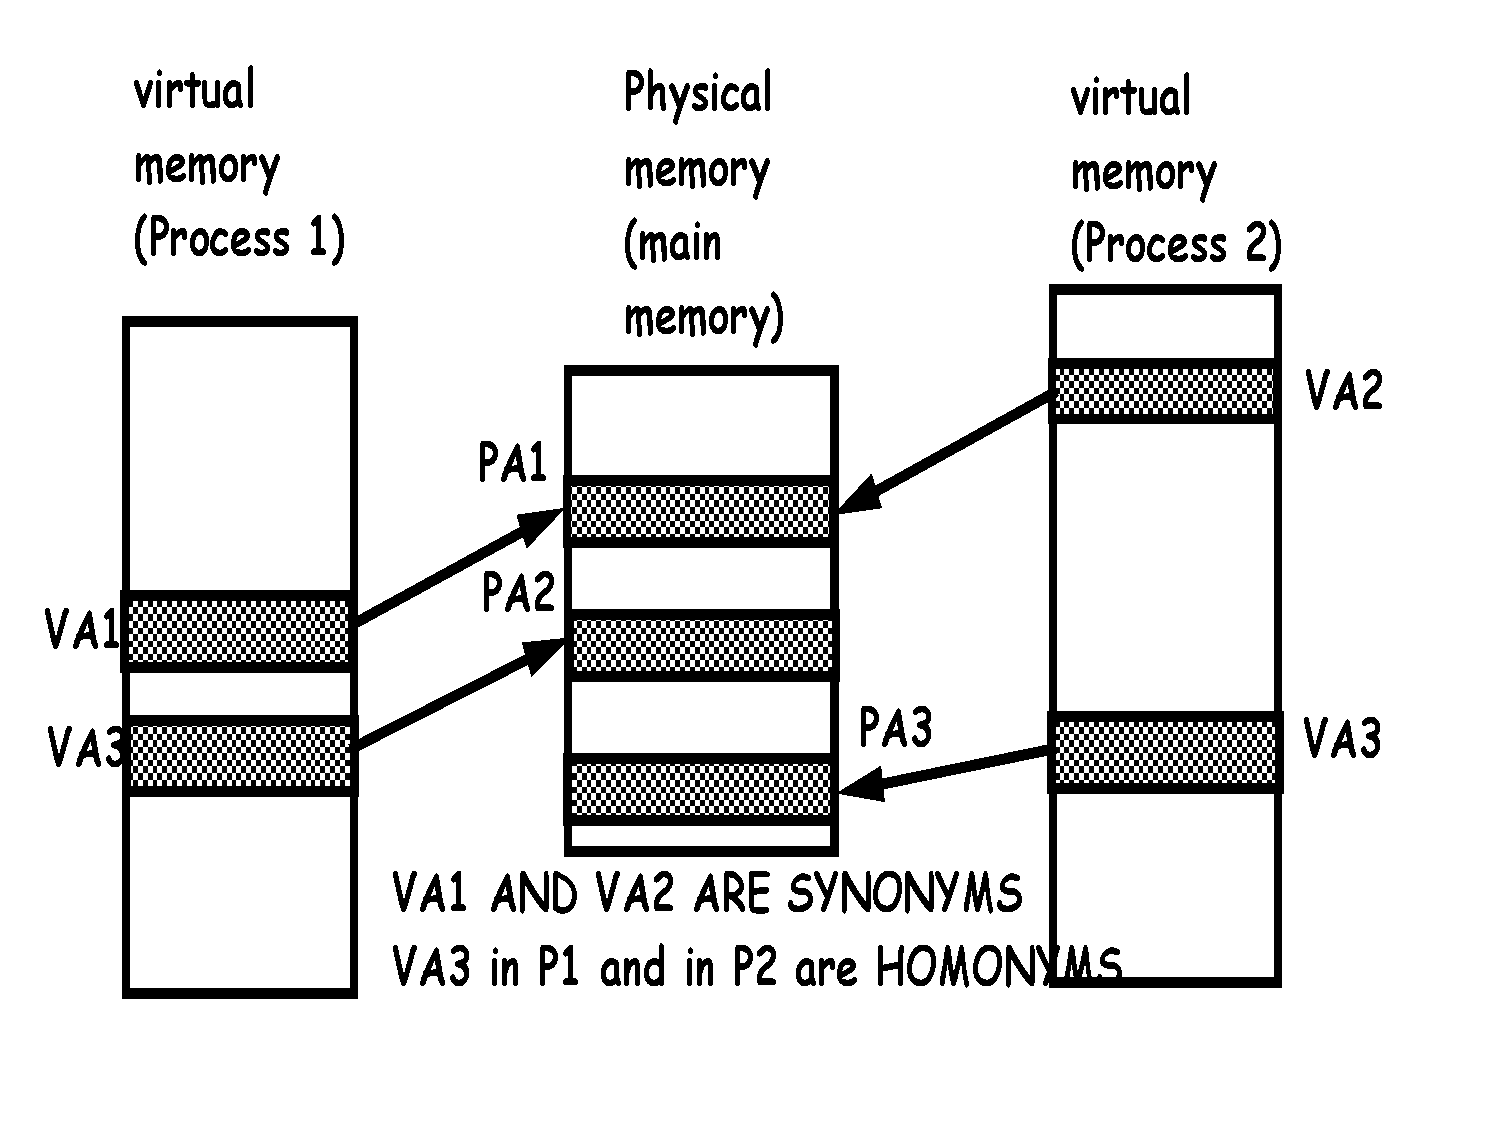
\includegraphics[width=55ex]{FigsMemH/PageSynHom}

\end{frame}

\begin{frame}[fragile,t]
\frametitle{Paged Virtual Memory}

\begin{itemize}
    \item Virtual address space divided into pages,\bigskip
    \item Physical address space divided into page frames,\bigskip
    \item Page Missing in Main Memory (MM) $\Rightarrow$ Page Fault
        \begin{itemize}
        %\begin{scriptsize}
            \item Pages not in MM are on disk: swapped-in/swapped-out,
            \item or have never been allocated.
            \item New page may be placed anywhere in MM (fully-associative)
        %\end {scriptsize}
        \end  {itemize}\bigskip
    \item Dynamic Address Translation:
        \begin{itemize}
        %\begin{scriptsize}
            \item Effective address is virtual, but
            \item must be translated to physical for every access.
            \item Virtual-to-physical address translation through page table in MM!
        %\end {scriptsize}
        \end  {itemize}
\end  {itemize}

\end{frame}


\begin{frame}[fragile,t]
\frametitle{Page Table}

\begin{columns}
\column{0.55\textwidth}
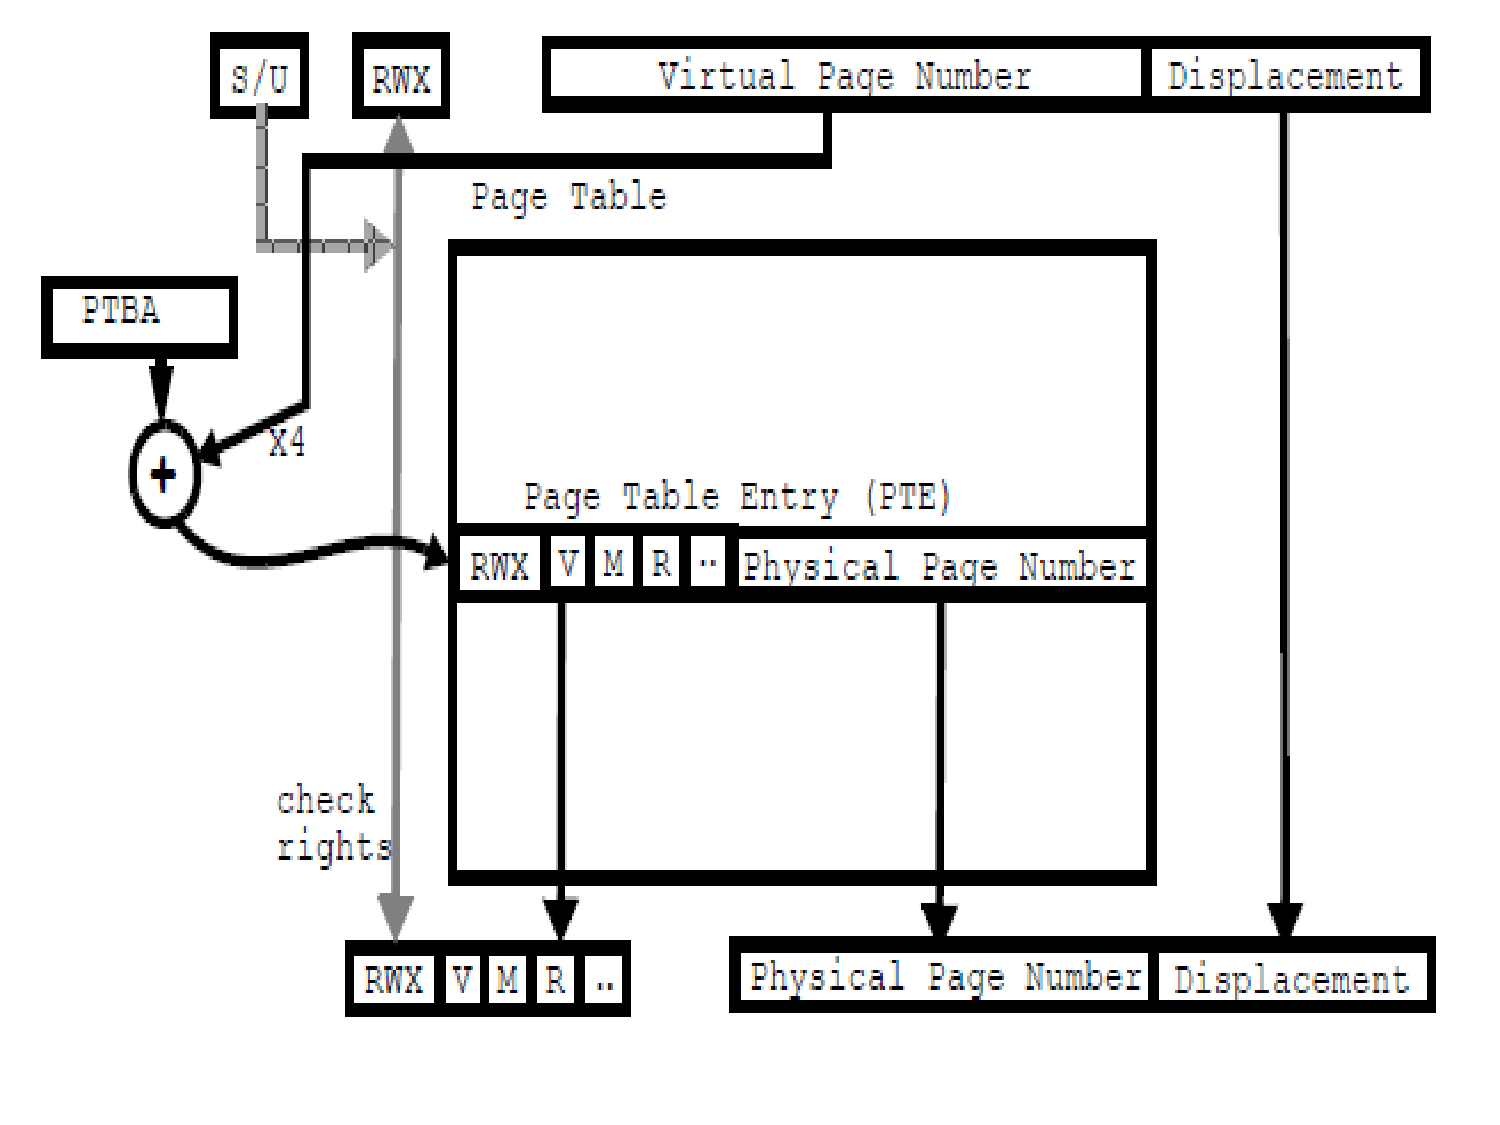
\includegraphics[width=40ex]{FigsMemH/PageTable}
\column{0.40\textwidth}
Translates Addresses \& Enforces Protection\smallskip

Page Replacement: FIFO--LRU--MFU
\end{columns}

Approximate LRU:
\begin{itemize}
\item Reference Bit (R) per page is periodically reset by OS.
\item Page Cached: hard vs soft page faults.
\end{itemize}\bigskip

Write-Back Strategy using Modify Bit (M);\\
M and R easily maintained by OS.

\end{frame}


\begin{frame}[fragile,t]
\frametitle{Hierarchical Page Table}

\begin{columns}
\column{0.55\textwidth}
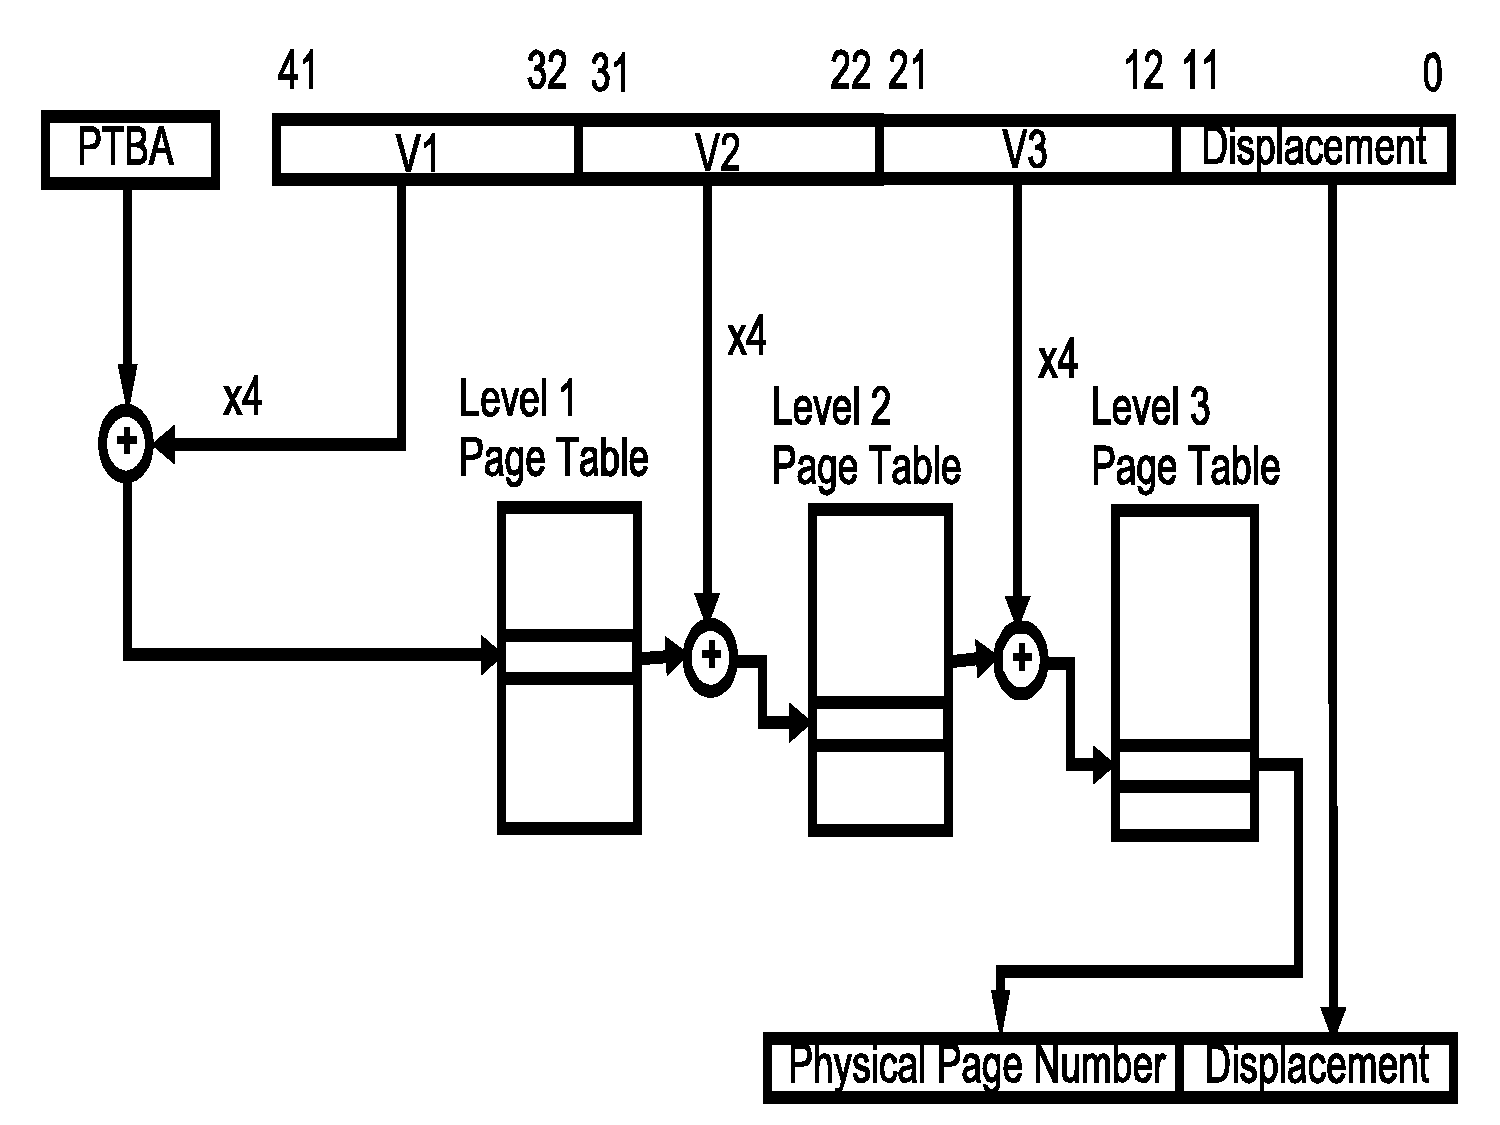
\includegraphics[width=40ex]{FigsMemH/HierarchPageTable}
\column{0.40\textwidth}
Supports SuperPages (How?)\smallskip


\end{columns}

Multiple DRAM access per memory translation:
\begin{itemize}
\item cached $\Rightarrow$ multiple cache accesses.
\item Solution: special cache dedicated to translations (TLB)
\end{itemize}\bigskip

\end{frame}

\begin{frame}[fragile,t]
\frametitle{Translation Lookahead Buffer (TLB)}

\begin{columns}
\column{0.55\textwidth}
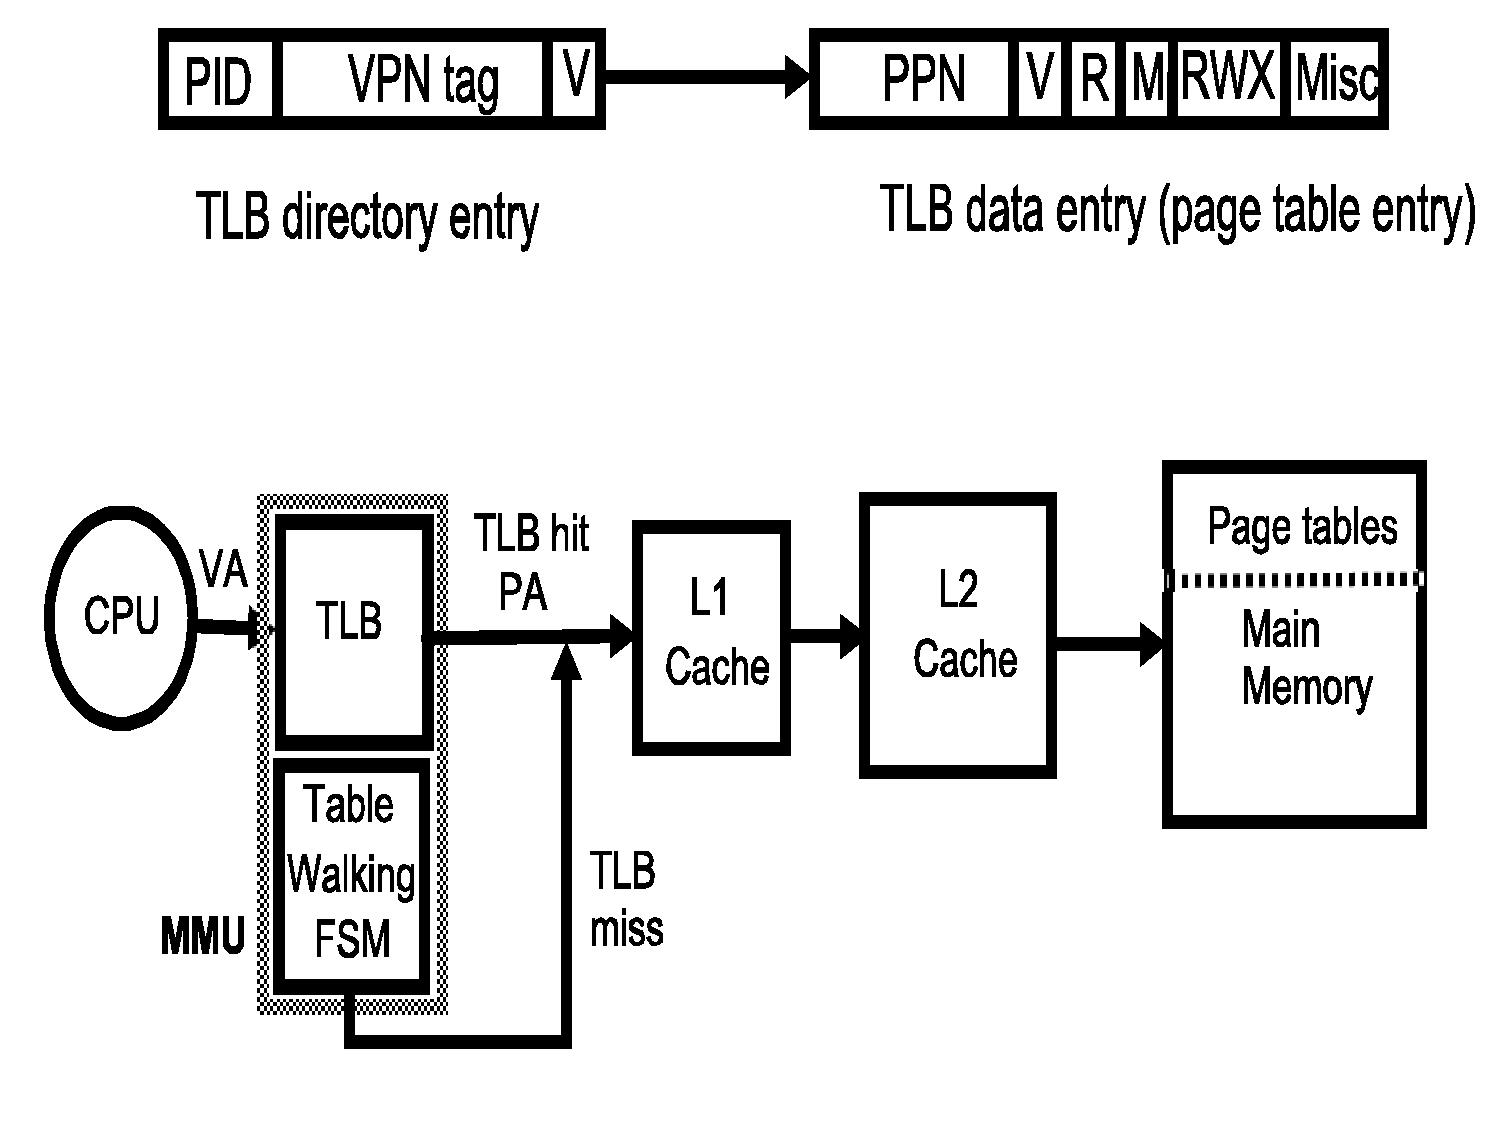
\includegraphics[width=40ex]{FigsMemH/TLB}
\column{0.40\textwidth}
Page Table Entries Are Cached in TLB:\\\smallskip
\begin{scriptsize}
TLB: DM/SA/FA cache accessed with VPN,\\
PID added to deal with homonyms.
\end{scriptsize}
\end{columns}

\begin{itemize}
\item TLBs $<<$ caches because of coverage.
\item iTLB and dTLB
\item TLB misses treated by ``table walking'' in 
\item Hardware MMU or software (trap handler).
\end{itemize}\bigskip

\end{frame}

\begin{frame}[fragile,t]
\frametitle{Optimizing TLB Access}


TLB is on the critical memory-access path:
\begin{itemize}
    \item pipeline: IF split into IF$_{TLB}$ \& IF$_{cache}$, same for ME stage
    \item access TLB in parallel with cache
        \begin{itemize}
            \item \emph{possible because of the two-step access}, but still
            \item \emp{L1 size is limited to 1 page per way of associativity. Why?}
        \end {itemize}
\end  {itemize}


\begin{columns}
\column{0.55\textwidth}
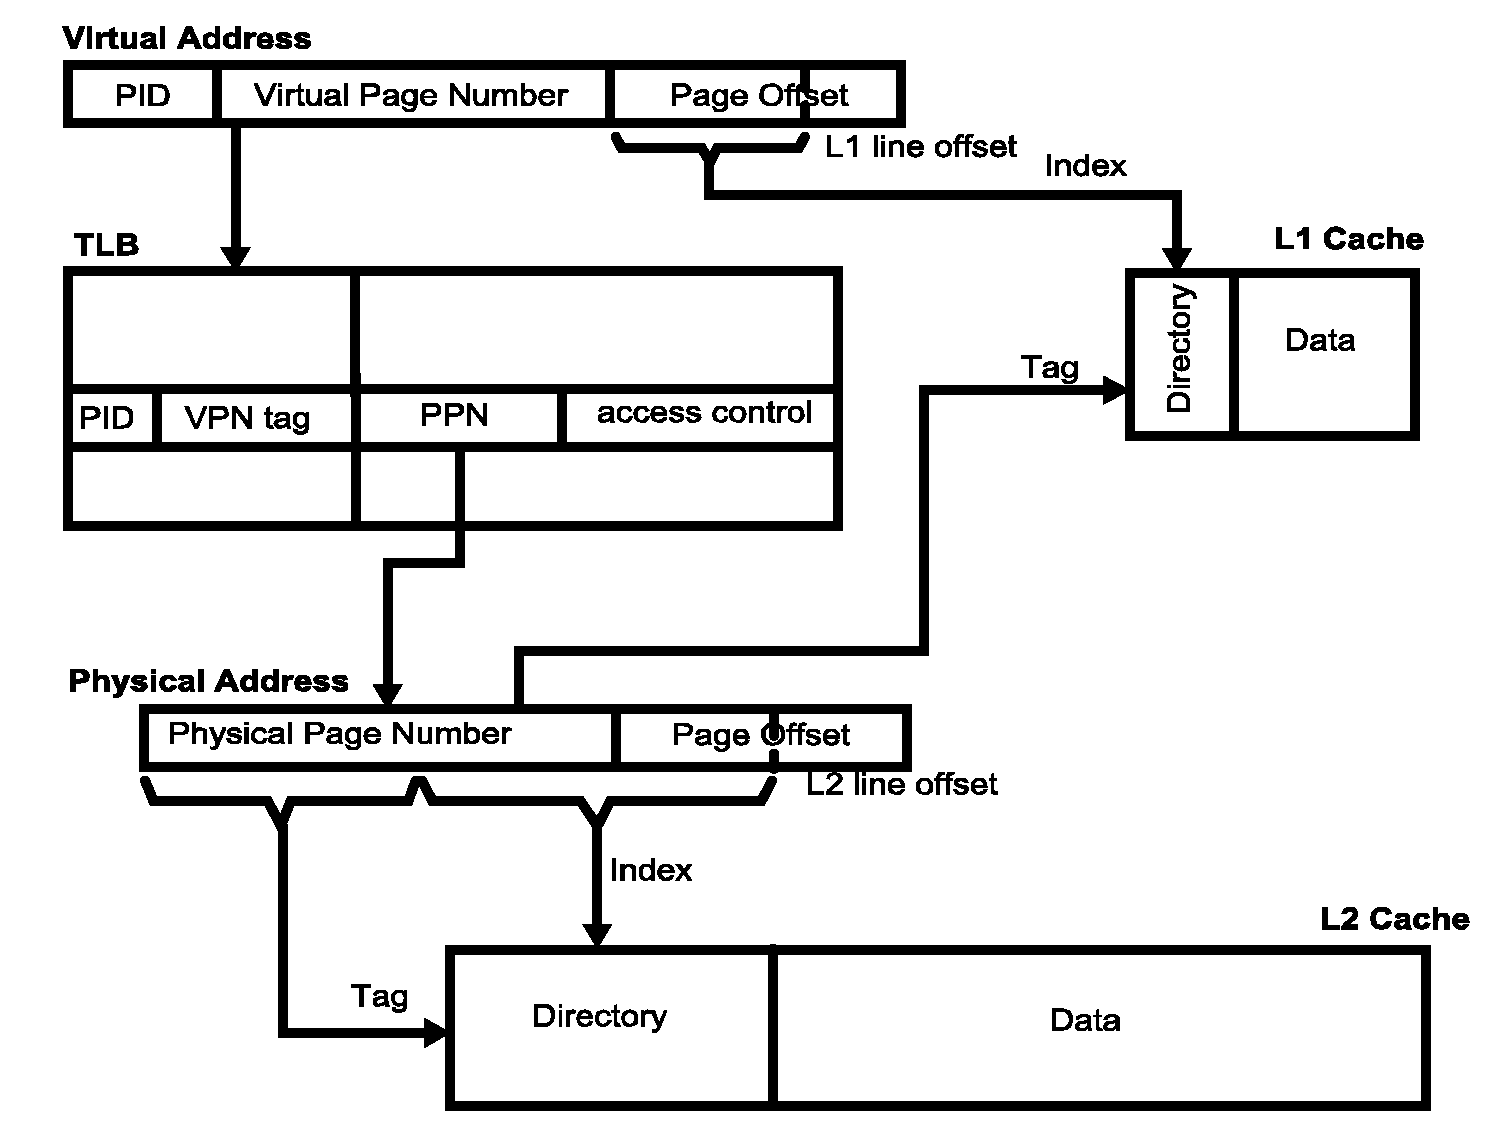
\includegraphics[width=40ex]{FigsMemH/TLBtransl}
\column{0.40\textwidth}
Need to use only bits in Page Offset to index in Directory.\\\bigskip

Otherwise: one block might be placed in two sets (due to synonyms).
\end{columns}

{\scriptsize Moving TLB after L1 cache, by indexing on the 
 virtual address $\Rightarrow$ many other problems!}


\end{frame}

\end{document}
